\section{Contextual Foundation}
\label{contextual_foundation}

This chapter establishes the foundational knowledge required for a comprehensive exploration of automated software testing in the context
 of an API. The section is divided into four subsections:

\begin{enumerate}
    \item Database: Examines the strengths and limitations of NoSQL databases, with a focus on MongoDB as a document store. 
    Key topics include scalability, schema flexibility, and the advantages of JSON/BSON for integration testing.
    \item HTTP Semantics: Explores the principles of HTTP as a stateless protocol, covering request-response models, status codes, 
    methods, and their relevance to API testing.
    \item Application Programming Interface: Introduces the design and architecture of the Medical Appointments Management API, 
    including \hyperref[appendix:glossary]{UML} class diagrams, modular monolith structure, and domain functionalities.
    \item Automated Software Testing: A critical component of software quality, consuming significant project time. It identifies issues, ensures system functionality, and meets user needs. Good tests cover diverse scenarios, prevent future problems, and are supported by tools for efficient execution. Types include manual and automated testing (e.g., unit and integration tests).
\end{enumerate}

The discussion bridges theoretical concepts with practical applications, emphasizing how these fundamentals underpin the development 
and testing of the API.

\subsection{Database}
\label{subsection:database}

Databases are an organized collection of data that enables the handling of large-scale datasets by inputting, storing, retrieving, 
and managing them. A database management system is defined as software that provides the interface between users and a database \cite{birgen2014sql}.

The \hyperref[appendix:glossary]{DBMS} has the responsibility of maintaining the integrity and security of the stored data. Furthermore, databases can be categorized into different criteria: i.e., when a database relies on tables to organize data, it is labeled as a \textit{relational}. Otherwise, when the database does not rely on tables, it is labeled as \textit{non-relational}. Besides, it is worth highlighting that non-relational databases are also 
known as \textit{NoSQL databases} \cite{birgen2014sql, jatana2012survey}.

For instance, \hyperref[appendix:glossary]{DBMS} relies on structured data organization using tables, schemata, columns, rows, primary keys, and foreign keys. 
Foreign keys are essential for establishing one-to-one, one-to-many, and many-to-many  relationships between entities \cite{bhat2010moving}.

The rigid data structure of \hyperref[appendix:glossary]{DBMS} often encounters scalability challenges with increasing data volumes and transaction loads, as included in the Table \ref{rdbms_challenges}: 

\begin{table}[H]
\centering
\caption{Relational Database Scalability Challenges}
\label{rdbms_challenges}
\begin{tabular}{p{0.45\textwidth}p{0.45\textwidth}}
\toprule
\textbf{Technical Challenges} & \textbf{Structural Limitations} \\
\midrule
Difficulty in predicting performance bottlenecks & Rigid table format complicates complex data modeling \\ \hline
Complex data integrity in shared environments & SQL joins become ineffective with growing datasets \\ \hline
Dual design needs (operational vs analytical) & \\
\bottomrule
\end{tabular}
\footnotesize Source: Adapated from \cite{bhat2010moving, jatana2012survey}.
\end{table}

These constraints underscore why NoSQL databases excel in handling large datasets where relational models falter, particularly for 
handling large datasets where a rigid relational model can impede performance \cite{moniruzzaman2013nosqldatabasenewera}.

Consequently, NoSQL databases are crucial for Big Data applications, enabling efficient storage and retrieval of massive datasets. Unlike \hyperref[appendix:glossary]{DBMS}, which complies with \hyperref[appendix:glossary]{ACID} (Atomicity, Consistency, Isolation, and Durability) properties,  NoSQL databases typically prioritize \hyperref[appendix:glossary]{BASE} (Basically Available, Soft State, and Eventual Consistency)  principles \cite{carronosql}.

\hyperref[appendix:glossary]{BASE} derives from the \hyperref[appendix:glossary]{CAP} (Consistency, Availability, Partition-tolerance) theorem. Due to the partial use of the theorem by selecting two of the three principles from the theorem, many NoSQL databases have relaxed the requirements to match their own needs on the consistency principle in order to achieve better availability and partitioning,  which resulted in the creation of \hyperref[appendix:glossary]{BASE} \cite{padhy2011rdbms}.

Scalability in distributed systems is closely tied to the \hyperref[appendix:glossary]{CAP} theorem and the \hyperref[appendix:glossary]{BASE} model. By prioritizing availability and partition tolerance over strict consistency, as facilitated by \hyperref[appendix:glossary]{BASE} principles, NoSQL databases enhance their ability to scale. This trade-off allows for efficient data distribution and workload management across multiple nodes, crucial for handling the demands of modern, large-scale applications \cite{brewer2012cap}.

Turning to scalability, it refers to an architecture's capacity to handle a growing number of components and interactions. This capacity is influenced by factors such as interaction frequency, load distribution (uniform vs. peak), delivery guarantees (assured vs. best-effort), request handling (synchronous vs. asynchronous), and environmental control (controlled vs. anarchic) \cite{fielding2000thesis}.

A key advantage of NoSQL's scalability is its ability to scale both vertically and horizontally. As another advantage, NoSQL databases are more suitable to store data across a cloud of servers. \cite{mason2015nosql, padhy2011rdbms} states that vertical scalability is done by adding resources to a single server. Horizontal scalability is achieved by distributing data across multiple servers. The dual scalability overcomes the vertical scalability limitations of traditional \hyperref[appendix:glossary]{SQL} databases.

In contrast with NoSQL's scalability, traditional \hyperref[appendix:glossary]{DBMS} scalability often involves expensive vertical scaling. The traditional \hyperref[appendix:glossary]{RDBMS} scalability is done by adding memory and CPU to servers. The adoption of NoSQL databases was largely driven by the high costs associated with scaling \hyperref[appendix:glossary]{DBMS} for large-scale data processing \cite{mason2015nosql, mohan2013history}.

As a consequence of the unaffordable costs associated with scaling \hyperref[appendix:glossary]{DBMS} for large-scale data processing, the cost-effectiveness and performance gains of NoSQL databases are primarily attributed to their distributed architecture, which utilizes inexpensive commodity servers \cite{mohan2013history}.

Building on these principles, NoSQL databases are categorized into the following types, as mentioned in the Table \ref{nosql_database_types}:

\begin{table}[H]
\centering
\caption{NoSQL Database Types}
\label{nosql_database_types}
\begin{tabular}{p{0.45\textwidth}p{0.45\textwidth}}
\toprule
\textbf{Primary Categories} & \textbf{Alternative Classifications} \\
\midrule
Key-value stores & Key-value pairs \\ \hline
Document stores & Document store \\ \hline
Column-family stores & Wide-column store \\ \hline
Graph databases &  \\ \hline
Column-oriented databases & Column-based databases \\ \hline
Object-oriented databases &  \\ \hline
Grid and cloud databases &  \\ \hline
XML databases &  \\ \hline
Multidimensional databases &  \\ \hline
Multi-value databases &  \\ \hline
Multi-model databases &  \\
\bottomrule
\end{tabular}
\footnotesize Source: Adapated from \cite{abramova2014nosql, cattell2011scalable, davoudianchenliu2018, jatana2012survey, mason2015nosql}.
\end{table}

Among these categories, key-value stores—the simplest NoSQL type—universally support insertion, deletion, and lookup operations while enabling scalability through distributed key management. Notably, document stores extend this model by encoding values as semi-structured documents (e.g., JSON or BSON), offering schema flexibility that allows runtime modifications
 \cite{abramova2014nosql, cattell2011scalable, davoudianchenliu2018}.

For instance, MongoDB is a prominent example of a document store NoSQL database. Document stores, like MongoDB, organize data in a hierarchical structure similar to \hyperref[appendix:glossary]{XML} documents \cite{agrawal2015survey, mason2015nosql}.

The figures \ref{fig:xml} and \ref{fig:mongodb} contain, respectively, examples of an \hyperref[appendix:glossary]{XML} and a MongoDB document.

\begin{figure}[H]
    \centering
    \caption{Example of XML Document}
    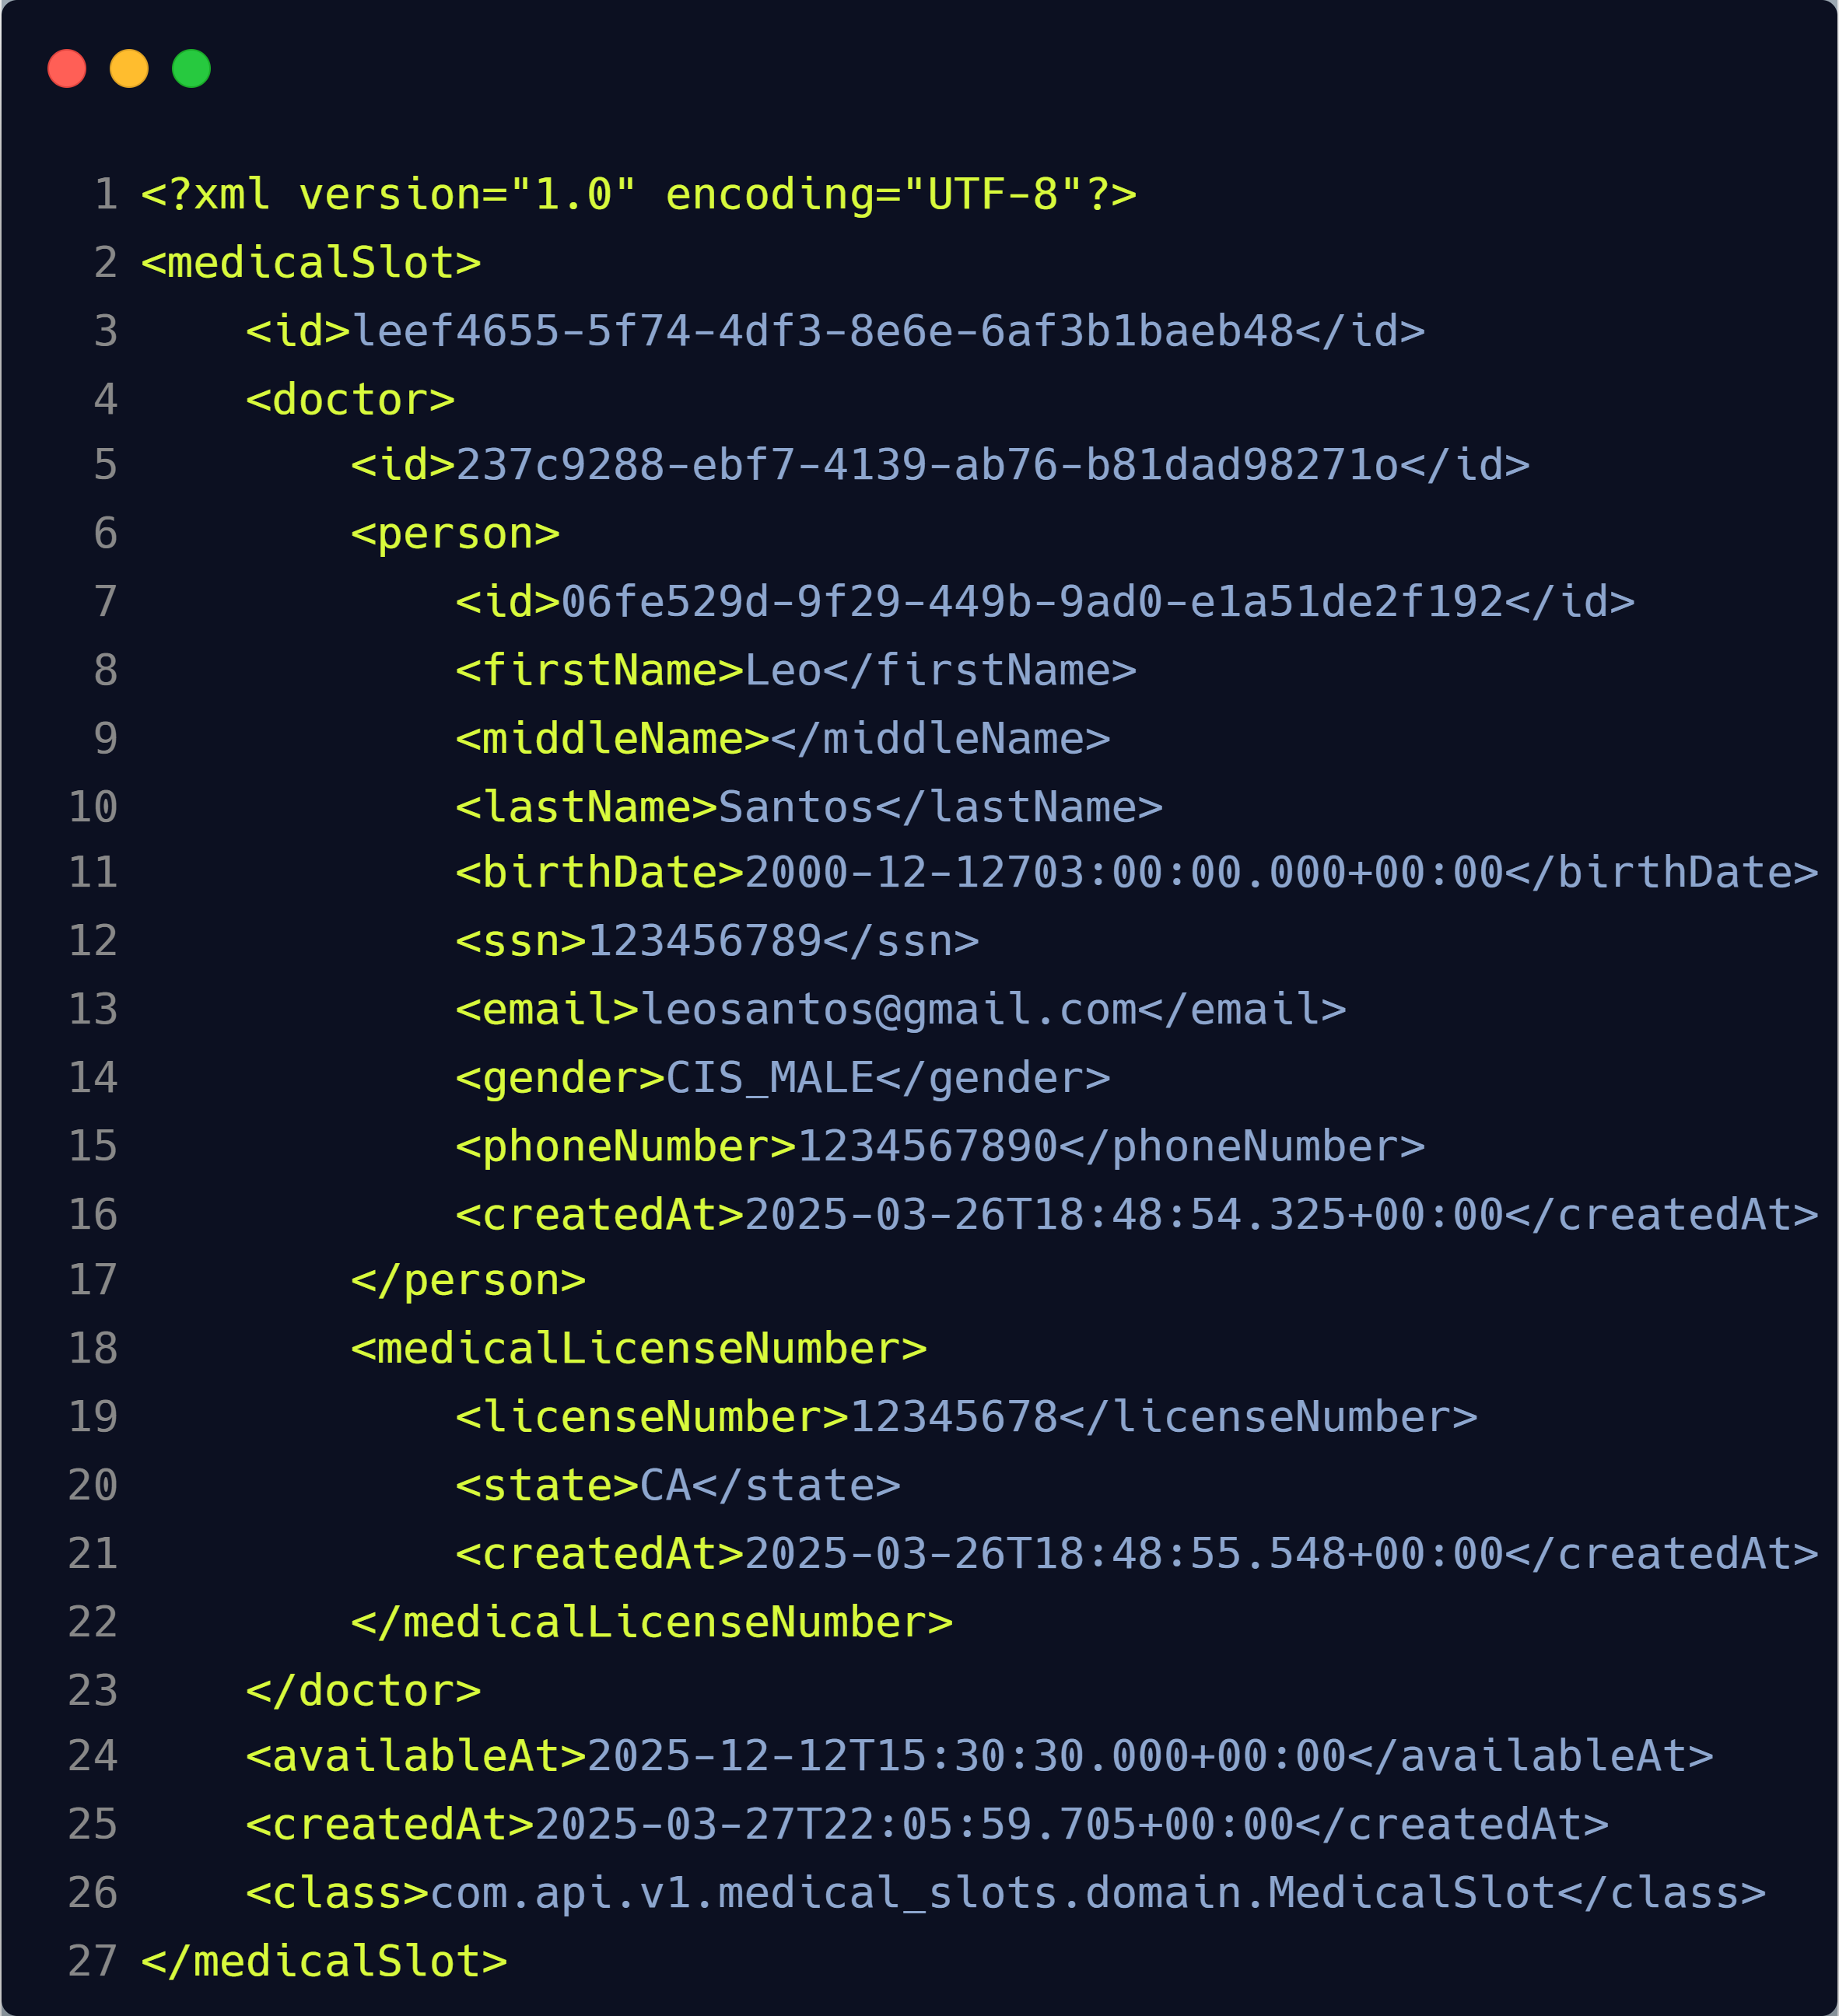
\includegraphics[width=1\linewidth]{figures/db/xml.png}
    \label{fig:xml}
    \footnotesize Source: Author's creation.
\end{figure}

\begin{figure}[H]
    \centering
    \caption{Example of MongoDB Document}
    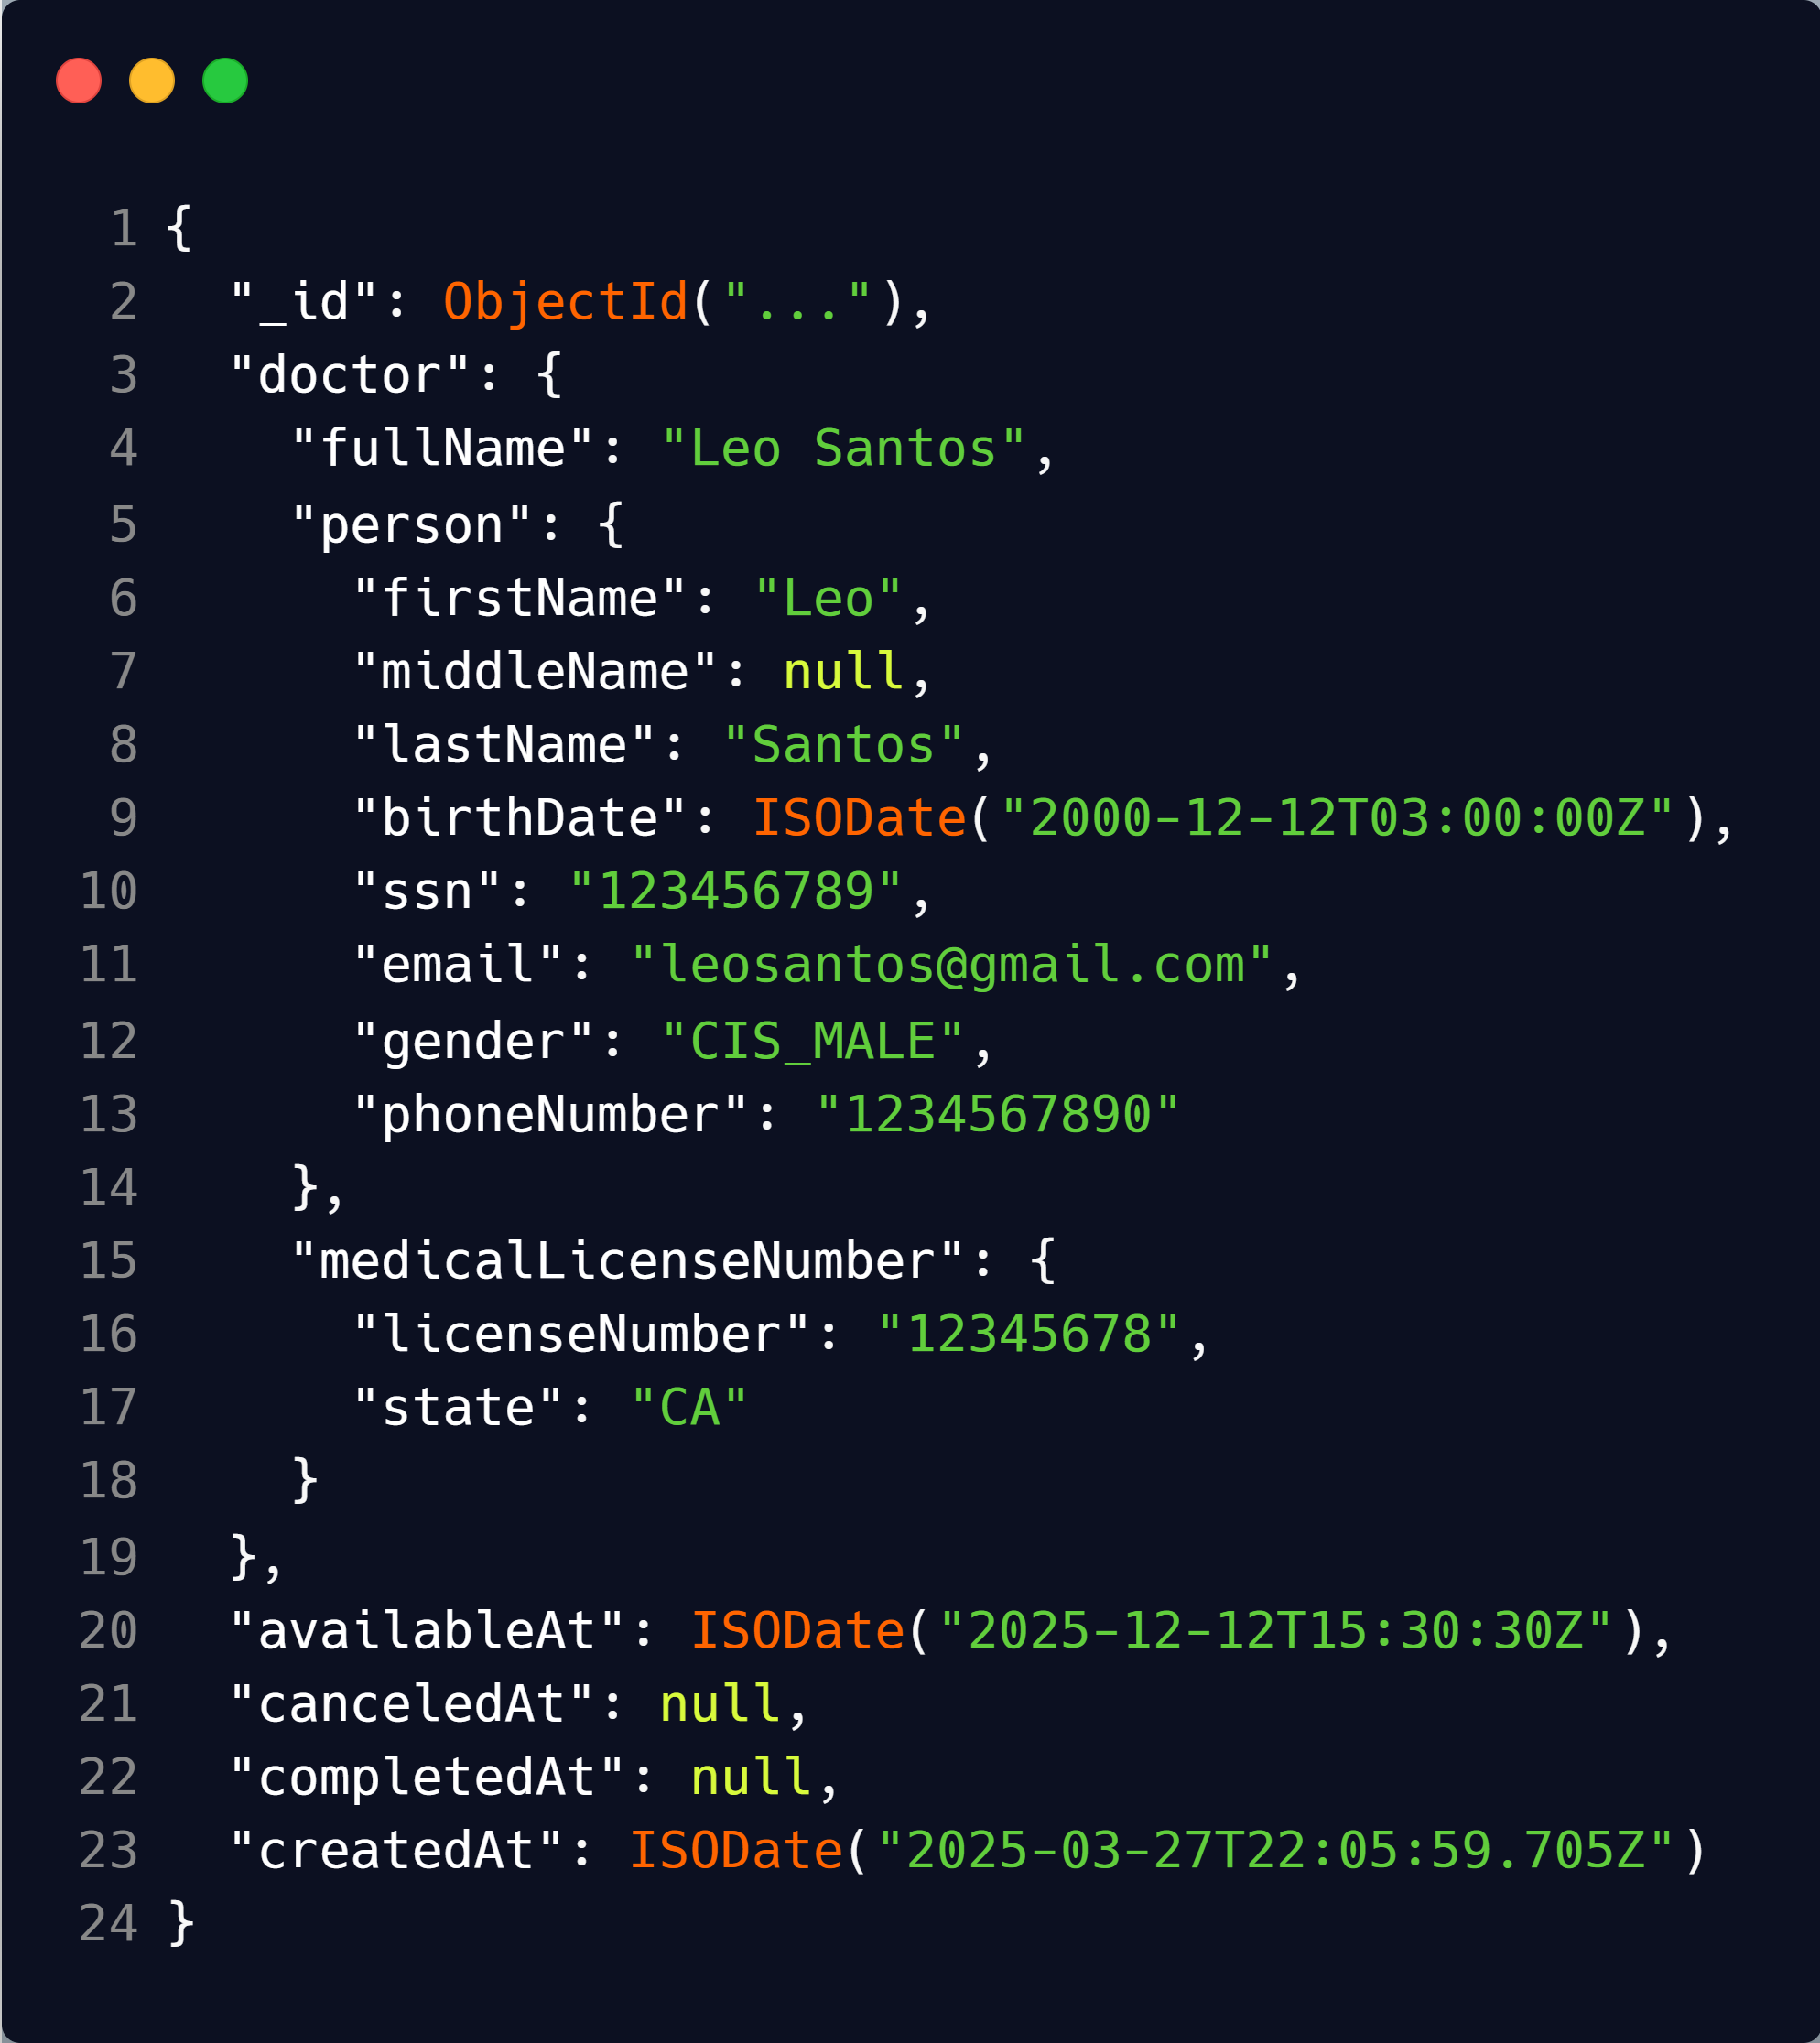
\includegraphics[width=1\linewidth]{figures/db/mongodb.png}
    \label{fig:mongodb}
    \footnotesize Source: Author's creation.
\end{figure}

It is noticeable the key-value structure in the shape of tags in figure \ref{fig:xml}. Such structure resembles the way the data  is organized in figure \ref{fig:mongodb}. Furthermore, there's a notable hierarchical structure in both figures.  As illustrated in figure \ref{fig:mongodb}, the embedded \textit{doctor} object that contains the embedded \textit{person} 
 and \textit{medicalLicenseNumber} objects within a single document demonstrates MongoDB's schema flexibility,  contrasting with the relational model's reliance on foreign key setting relationships. Notably, MongoDB has some key strengths and weaknesses described in the Table \ref{mongodb_strenghts_weaknesses}:

\begin{table}[H]
\centering
\caption{MongoDB Strengths and Weaknesses}
\label{mongodb_strenghts_weaknesses}
\begin{tabular}{p{0.45\textwidth}p{0.45\textwidth}}
\toprule
\textbf{Strengths} & \textbf{Weaknesses} \\
\midrule
Sharding capability & No native join operations \\ \hline
High speed performance & Absence of transactions \\ \hline
Efficient storage and distribution of large binary files & Historically immature platform \\ \hline
Fault tolerance policy & No standardized query language \\ \hline
Complex query language & Complex query language may be difficult for users \\ \hline
Open-source nature & Consistency compromise may cause issues for sensitive transactions \\ \hline
Better performance and scalability when consistency is compromised & \\ \hline
No requirement for a predefined model or structure for data storage & \\
\bottomrule
\end{tabular}
\footnotesize Source: Adapated from \cite{agrawal2015survey, hajoui2018nosql, jatana2012survey, leavitt2010will, mason2015nosql, nayak2013type}.
\end{table}


Additionally to what was mentioned in the Table \ref{mongodb_strenghts_weaknesses}, document store databases offer schema flexibility, allowing documents within a collection to have varying local schemata. While this flexibility supports agile development, it requires careful data management to prevent inconsistencies due to the absence of enforced schema constraints \cite{gallinucci2018schema}. JSON is a lightweight data-interchange format whose strengths are described in the Table \ref{json-characteristics}: 

\begin{table}[H]
\centering
\caption{JSON Characteristics}
\label{json-characteristics}
\begin{tabular}{p{0.45\textwidth}p{0.45\textwidth}}
\toprule
\textbf{Advantages} & \textbf{Features} \\
\midrule
Straightforward readability for humans and machines & 
Uses familiar conventions of C-languages \\ \hline
Feasible to write and generate & 
Compatible with C-inspired languages (Java, JavaScript, etc.) \\ \hline
Text format independent of any programming language & 
Straightforward format of name-value pairs \\ \hline
Simple data interchange format & Supports ordered lists of values \\
\bottomrule
\end{tabular}
\footnotesize Source: Adapated from \cite{jsonintroduction2025}.
\end{table}

The figure \ref{fig:json} provides an example of a JSON document that illustrates the straightforward readability, 
familiar C-language conventions, and straightforward name-value pair format.

\begin{figure}[H]
     \centering
     \caption{Example of JSON Document}
     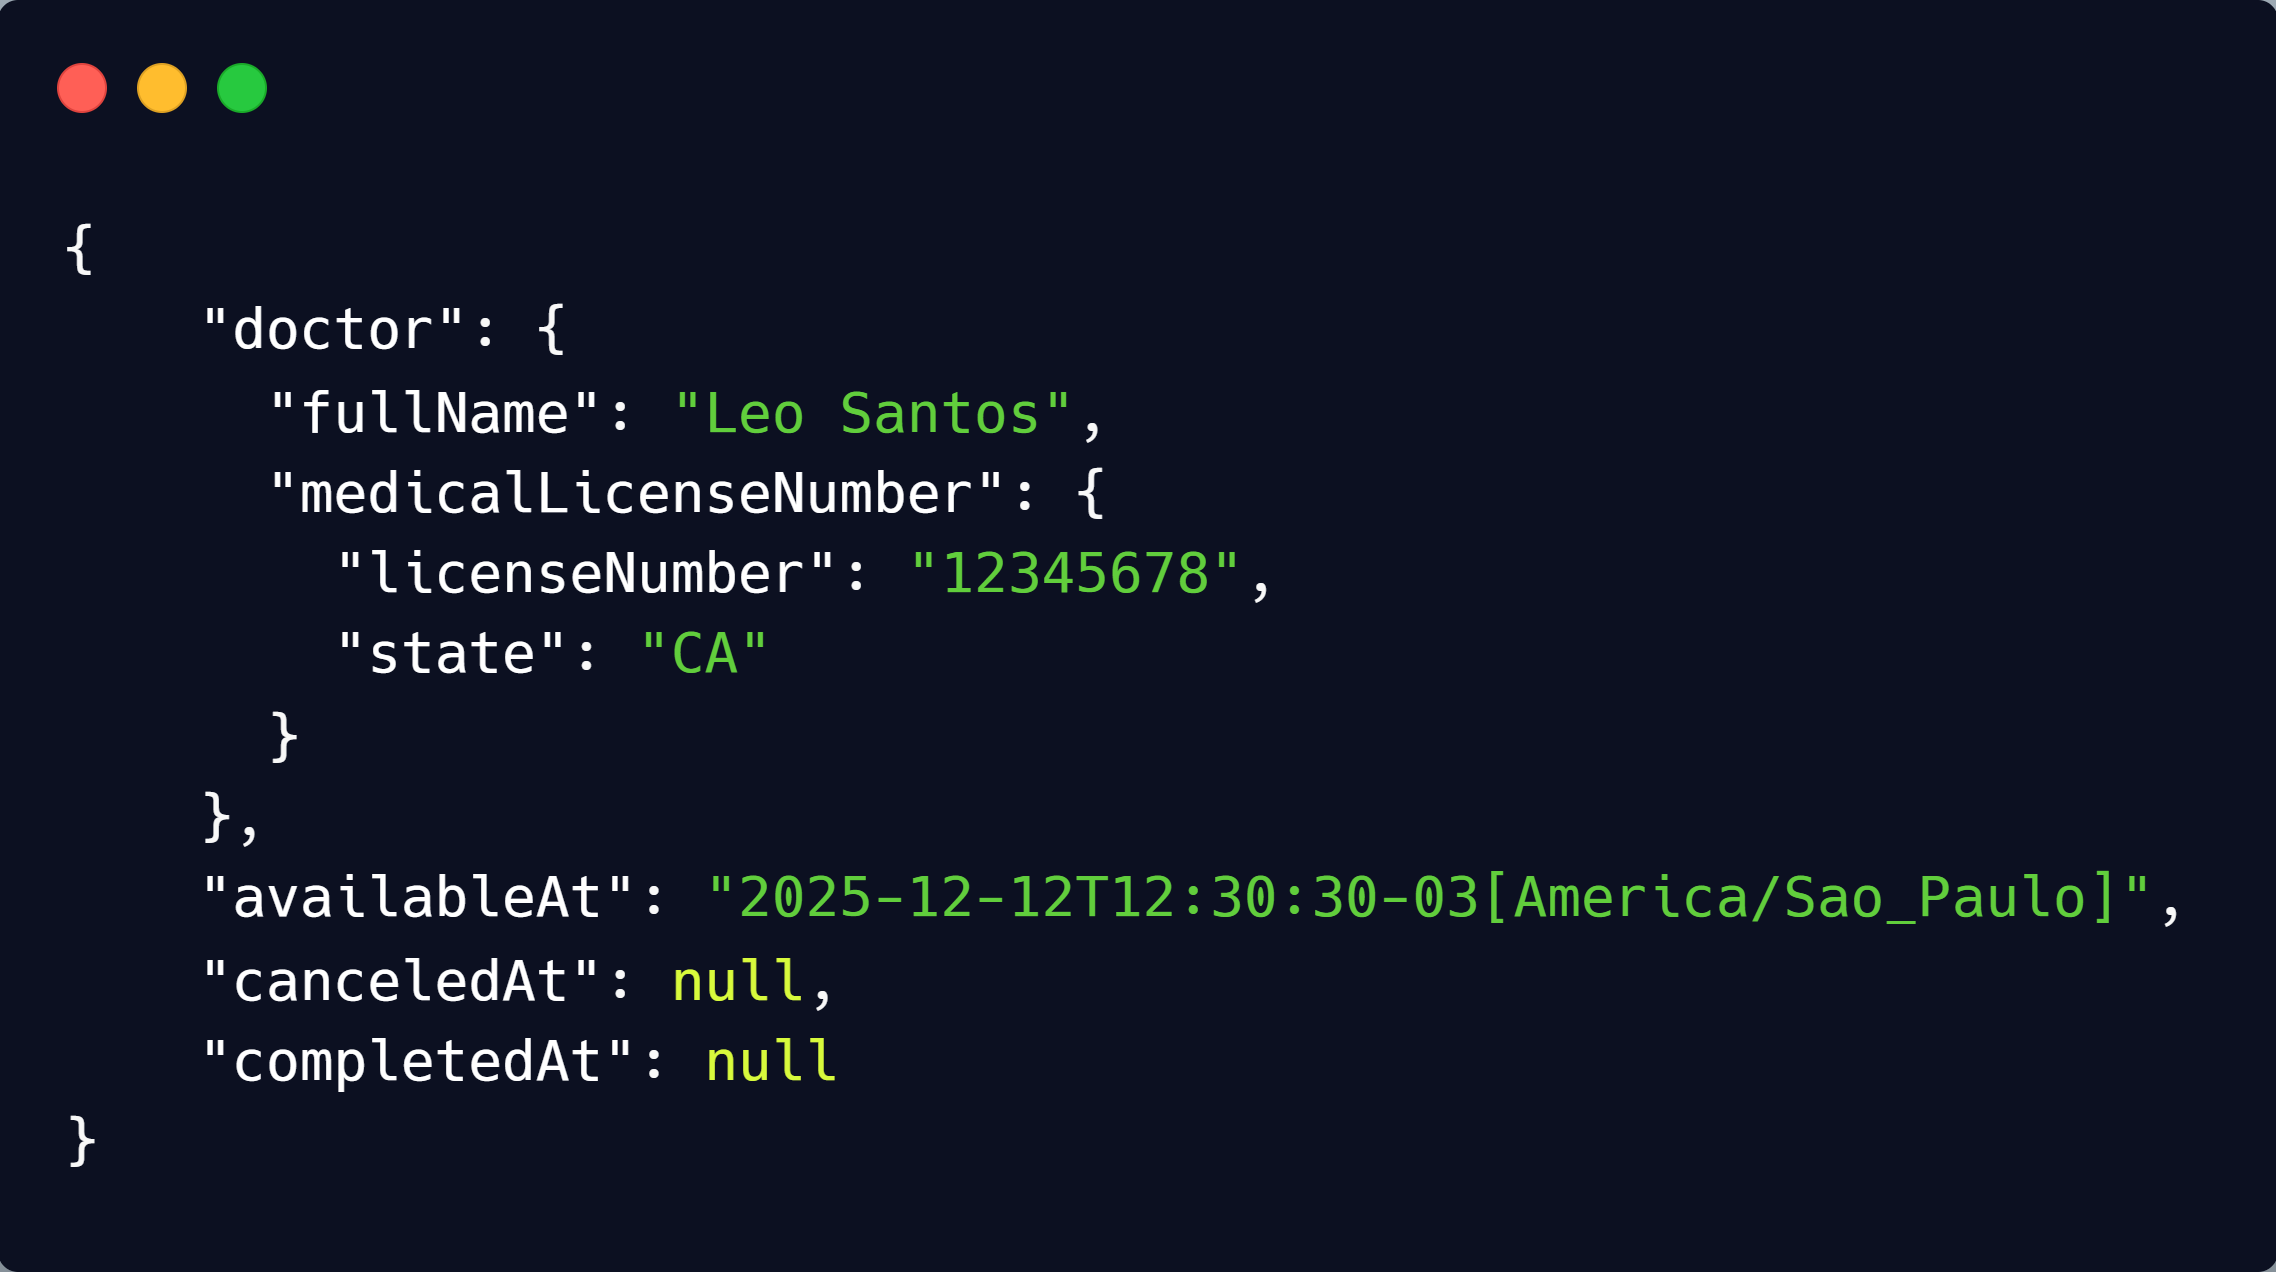
\includegraphics[width=1\linewidth]{figures/db/json.png}
     \label{fig:json}
     \footnotesize Source: Author's creation
\end{figure}

As displayed in the figure \ref{fig:json}, the structure of the JSON is unambiguous. The use of curly and square brackets to delimit where the JSON commences and finishes is a clear manner of organization. \cite{chasseur2013enabling} highlights that the format is used by MongoDB to store collections of JSON objects in lieu of relational tables, and JSON is used as the primary data format to interact with applications.

For instance, even though there is a resemblance between JSON and \hyperref[appendix:glossary]{XML}, and even their shared hierarchical semi-structured data model, JSON is indeed the replacement of \hyperref[appendix:glossary]{XML} due to JSON's simplicity, compactness, and the use of JS as the mapping language used to map data \cite{chasseur2013enabling}.
 
 As a consequence of a good product, BSON was created to suit the need of traversability of MongoDB in its primary data representation. Similar to JSON, BSON is lightweight, efficient, a binary-encoded serialization of JSON-like documents that supports embedding documents and arrays. Due to MongoDB's adoption of an extended key-value store, BSON holds data in a binary format in which zero or more ordered key/value pairs are stored as a single document \cite{bsonspecimplementation2025, bsonspec2025, bsonspecversion112025, davoudianchenliu2018}. 
 
One example of the mentioned key-value structure is shown in the figure \ref{fig:mongodb}.
 
Considering all the benefits of NoSQL and MongoDB, therefore in the context of automated software testing, MongoDB's flexible schema and document-oriented structure offer significant advantages for integration testing. The ability to easily insert and persist embedded documents in BSON format directly reflects the successful execution of integration tests.

\subsection{HTTP Semantics}
\label{subsection:http_semantics}

HTTP, a stateless application-layer protocol, uses a request-response model and self-descriptive messages for flexible hypermedia communication.
 It provides a uniform interface, abstracting resource access, and serves as the primary  Web communication protocol for resource representation
  transfer \cite{rfc9110, fielding2000thesis}.

Within this framework, communication is structured around messages, which are categorized as either requests or responses. A client initiates interaction by constructing request messages that articulate its intentions and are directed to a designated server \cite{rfc9110}.

The server performs the following steps mentioned in the list below, as evidenced by \cite{rfc9110}:

\begin{enumerate}
    \item Listens for requests;
    \item Parses each received message;
    \item Interprets message semantics relative to the target resource;
    \item Responds with one or more response messages.
\end{enumerate}

Once these steps are completed, the client evaluates the response’s status code to verify successful execution and determines subsequent actions, 
as defined by HTTP semantics \cite{rfc9110}.

Moreover, in order to identify resources across HTTP, \hyperref[appendix:glossary]{URI} references are used to target requests, indicate redirects, and define relationships.
Despite any regulation issued by \hyperref[appendix:glossary]{IANA}\footnote{\href{https://www.iana.org/about}{See about IANA.}}, 
the HTTP server has two inherent schemes, as demonstrated by the Table \ref{tab:http-server-schemes}: 

\begin{table}[H]
\centering
\caption{HTTP server schemes}
\label{tab:http-server-schemes}
\begin{tabular}{lll}
\textbf{Scheme} & \textbf{Full Name} & \textbf{Example} \\ \hline
http & Hypertext Transfer Protocol & "http" "://" authority path-abempty {[} "?" query {]} \\ \hline
https & Hypertext Transfer Protocol  Secure & "https" "://" authority path-abempty {[} "?" query {]} \\ \hline
\end{tabular}
\\ \footnotesize Source: Adapated from \cite{rfc9110}.
\end{table}

In relation to the http schemes, the resource relies on the scheme to route its message to the appropriate server and port. The schemes allow the request to be listened to by the correct server and return the actual result to the client.

Turning to the status codes, as stated by \cite{rfc9110}, the status code of a response is a three-digit integer code within 100 to 599 that describes the result of the request and the semantics of the response, as well as the success or failure of the request and what content is enclosed. In order to facilitate the comprehension of the status codes, only their first digit 
categorizes the response's class \cite{rfc9110}.

Thus, the status codes are divided into 5 categories, as shown below in the Table \ref{tab:http-status-codes-simplified}:

\begin{table}[H]
\centering 
\caption{HTTP Status Codes}
\label{tab:http-status-codes-simplified}
\begin{tabular}{lll}
\textbf{Status code} & \textbf{Description} & \\ \hline
1xx & The request was received, continuing process & \\ \hline
2xx & The request was successfully received, understood, and accepted & \\ \hline
3xx & Further action needs to be taken in order to complete the request & \\ \hline
4xx & The request contains bad syntax or cannot be fulfilled & \\ \hline
5xx & The server failed to fulfill an apparently valid request & \\ \hline
\end{tabular}
\\ \footnotesize Source: Adapated from \cite{rfc9110}.
\end{table}

A more granular detailing of all status codes is described in the Appendix \ref{appendix:http_status_codes_summary_appendix}.

Furthermore, HTTP uses standardized request methods, independent of specific resources, for uniform network interactions.While the method's meaning remains consistent, resource implementation varies. The Table \ref{tab:http-methods} explains what each HTTP method does.

\begin{table}[H]
\centering
\caption{HTTP Methods}
\label{tab:http-methods}
\begin{tabular}{lp{6cm}} % Adjust the width (e.g., 6cm) as needed
\textbf{Method Name} & \textbf{Description} \\ \hline
GET & Transfer a current representation of the target resource. \\ \hline
HEAD & Same as GET, but do not transfer the response content. \\ \hline
POST & Perform resource-specific processing on the request content. \\ \hline
PUT & Replace all current representations of the target resource with the request content. \\ \hline
DELETE & Remove all current representations of the target resource. \\ \hline
CONNECT & Establish a tunnel to the server identified by the target resource. \\\hline
OPTIONS & Describe the communication options for the target resource. \\ \hline
TRACE & Perform a message loop-back test along the path to the target resource. \\ \hline
\end{tabular}
\\ \footnotesize Source: Adapated from \cite{rfc9110}.
\end{table}

In order to complement the table above and the function of the status codes (Table \ref{tab:http-status-codes}) of displaying the response's status to the client, the HTTP methods indicate the action expected from the execution of the request made by the client. Thus, below is an example of a resource that requests the registration of a doctor in the figure \ref{fig:http-request} and the service class that supports it in the figure \ref{fig:medical_slot_registration_service}.

\begin{figure}[H]
    \caption{Example of a HTTP request and response}
    \centering
    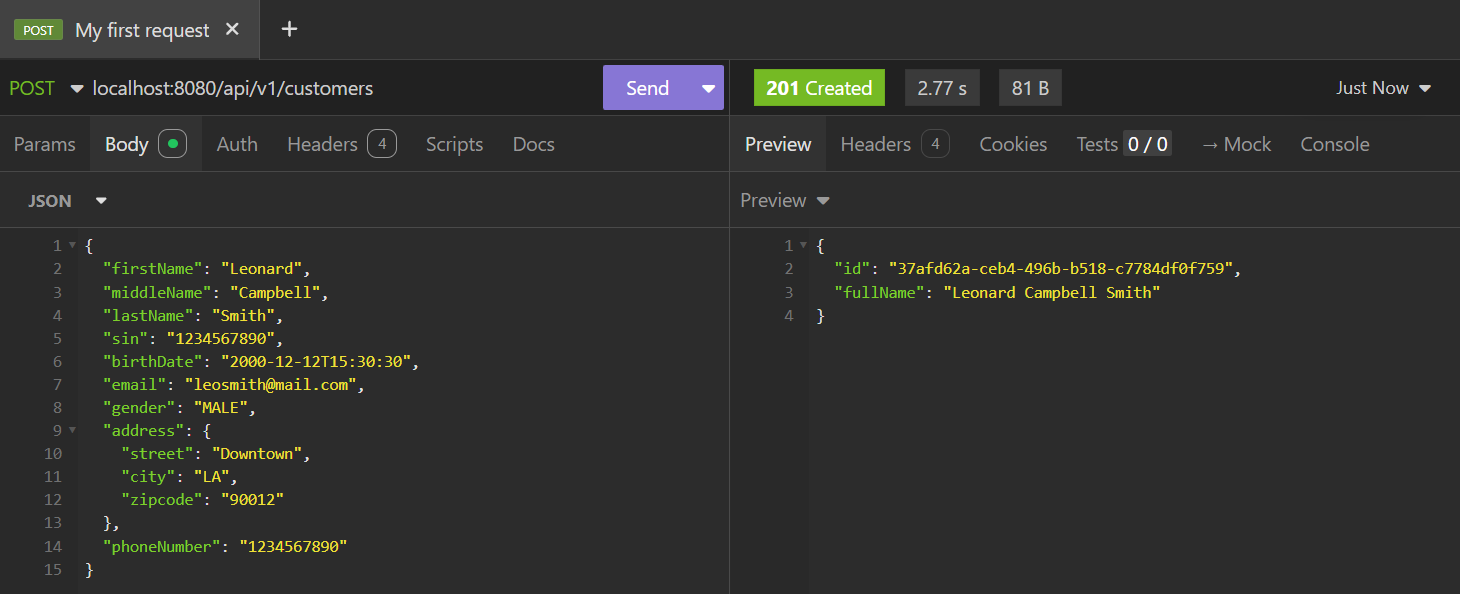
\includegraphics[width=1\linewidth]{figures/http/http_request_response.png}
    \label{fig:http-request}
    \footnotesize Source: Author's creation
\end{figure}

 \begin{figure}[H]
    \centering
    \caption{Example of a Registration Service}
    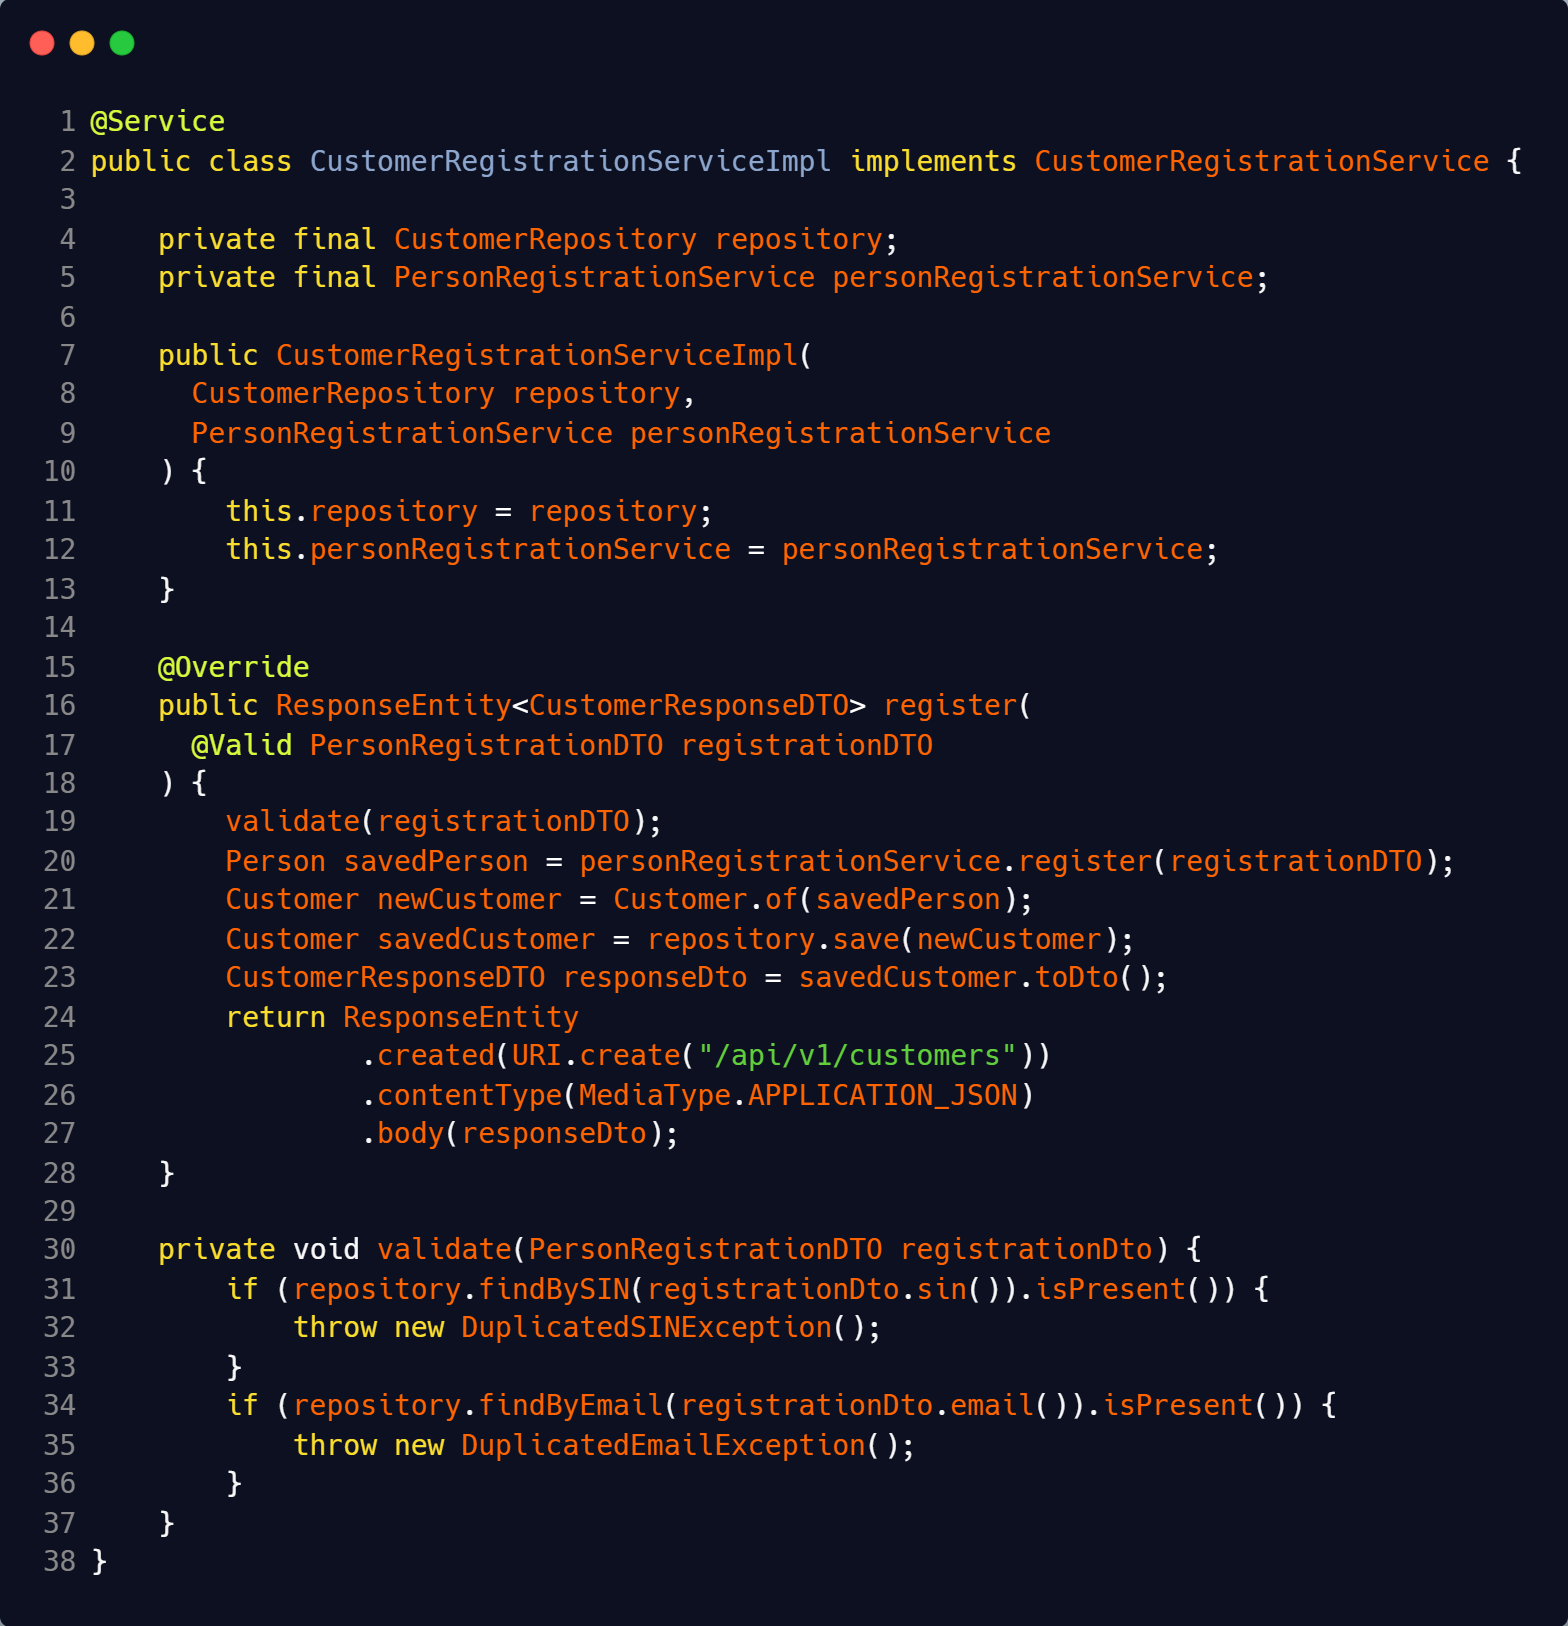
\includegraphics[width=0.83\linewidth]{figures/http/customer_registration_service_impl.png}
    \label{fig:customer_registration_service_impl}
    \\ \footnotesize Source: Author's creation.
\end{figure}

As exposed by the figure \ref{fig:http-request}, the POST method was used alongside the \hyperref[appendix:glossary]{URI} that was mentioned in the given figure. It follows the structure presented by the Table \ref{tab:http-server-schemes}, especially the \textbf{http}'s scheme. The service's code shown by the figure \ref{fig:customer_registration_service_impl} demonstrates the resource returns the \hyperref[tab:summary_http_status_codes]{status code 201}. 

The figure \ref{fig:http_header} illustrates the header cited in the \href{https://www.rfc-editor.org/rfc/rfc9110.html#name-post}{subsection 9.3.3} of the \hyperref[appendix:glossary]{RFC} \href{https://www.rfc-editor.org/rfc/rfc9110.html}{9110}.

\begin{figure}[H]
	\centering
	\caption{Example of a Header}
	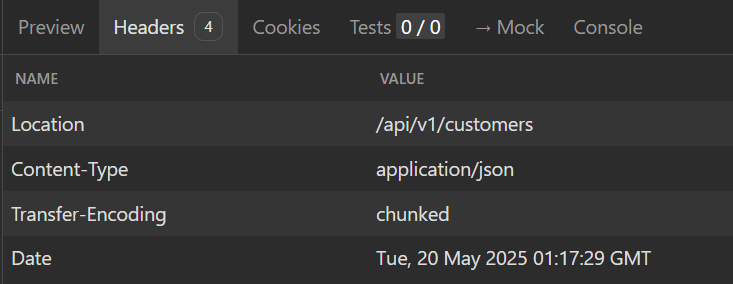
\includegraphics[width=0.9\linewidth]{figures/http/http_header.png}
	\label{fig:http_header}
	\\ \footnotesize Source: Author's creation.
\end{figure}

Moreover, the content in the figure \ref{fig:http_header}, there is a header location that can be used as an identifier for a specific resource corresponding to the representation in this message's content, as determined by \cite{rfc9110}. Therefore, this decision is aligned with \hyperref[appendix:glossary]{RFC} \href{https://www.rfc-editor.org/rfc/rfc9110.html}{9110}, especially in the \href{https://www.rfc-editor.org/rfc/rfc9110.html#name-post}{subsection 9.3.3}, as determined by \cite{rfc9110}, which emphasizes that the POST method is supposed to work with the \hyperref[tab:summary_http_status_codes]{status code 201} when the operation is successful.

Finally, in relation to automated software testing, the integration tests are going to behave as stated in the
Table \ref{tab:related-statuses-methods}:

\begin{table}[H]
\centering  
\caption{HTTP Method Status Code Outcomes}   
\label{tab:related-statuses-methods}    
\begin{tabular}{lll}
\textbf{HTTP Method} & \textbf{HTTP Status Codes When Successful} & \textbf{HTTP Status Codes When Failure} \\   
\hline   
GET & 200 & 400 or 404 \\ \hline   
POST & 201 & 400 or 409 \\ \hline   
PUT & 200 or 204 & 400 or 404 \\ \hline   
PATCH & 200 or 204 & 400 or 404 \\ \hline   
DELETE & 204 & 404 \\ \hline   
\end{tabular}  
\\ \footnotesize Source: Adapated from \cite{rfc9110}.
\end{table}

In the case of an integration test whose methods are PUT or PATCH, preference shall be given to the status code \hyperref[tab:summary_http_status_codes]{204}; 
unless \hyperref[appendix:glossary]{HATEOAS} is inserted into the resource's response, the chosen status code is \hyperref[tab:summary_http_status_codes]{200}. Therefore, the figure \ref{fig:http-methods-intenteded-content} displays the intended meaning of the content.

\begin{figure}[H]
    \centering
    \caption{HTTP Methods's Intended Content Meaning}
    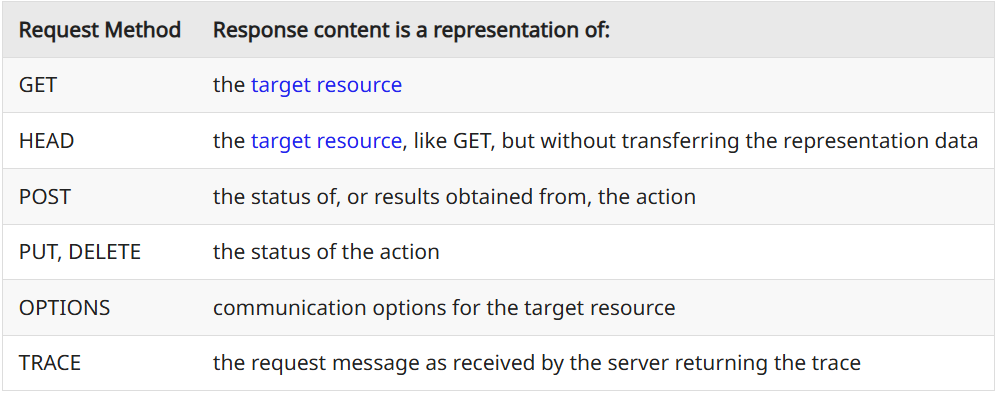
\includegraphics[width=1\linewidth]{figures/http/http_200_response_analyses.png}
    \label{fig:http-methods-intenteded-content}
    \footnotesize Souce: \cite{rfc9110}.
\end{figure}

As illustrated in figure \ref{fig:http-methods-intenteded-content}, the GET and POST methods are the only HTTP methods whose response content directly represents the target resource. In contrast, methods like PUT and DELETE primarily focus on conveying the status of the action rather than resource content. Meanwhile, OPTIONS and TRACE do not concern themselves with either the target resource or the status code in the same way. The HEAD method is similar to GET in that its metadata describes the target resource, but it intentionally omits the actual content transfer.

Given these distinctions, GET and POST are the most suitable choices for \hyperref[appendix:glossary]{HATEOAS} implementations, as they align with the principles outlined in \hyperref[appendix:glossary]{RFC} \href{https://www.rfc-editor.org/rfc/rfc9110.html}{9110}. While developers technically have the flexibility to use any HTTP method in \hyperref[appendix:glossary]{HATEOAS}, adhering to the standard ensures consistency, interoperability, and compliance with \hyperref[appendix:glossary]{RESTful} design best practices.

Additionally, proper use of HTTP status codes is critical for clear API semantics, as displayed by the Table \ref{http_error_codes}:

\begin{table}[H]
\centering
\caption{HTTP Status Code Semantics for Error Handling}
\label{http_error_codes}
\begin{tabular}{p{0.15\textwidth}p{0.8\textwidth}}
\toprule
\textbf{Status Code} & \textbf{Usage Context} \\
\midrule
409 & Request conflicts with server state (e.g., duplicate data in PUT requests: SSN, email, or medical license number) \\ \hline
404 & Requested resource does not exist \\ \hline
400 & Fallback for client errors not covered by 404/409 (e.g., malformed syntax or invalid parameters) \\
\bottomrule
\end{tabular}
\\ \footnotesize Source: Adapated from \cite{rfc9110}.
\end{table}

It is evident that the \hyperref[tab:summary_http_status_codes]{status code 400} is the default behavior when failure occurs. Hence, the importance of using specific status
 codes for specific situations highlights the impactful use of the status \hyperref[appendix:http_status_codes_summary_appendix]{404} and \hyperref[appendix:http_status_codes_summary_appendix]{409}.

\subsection{Application Programming Interface}
\label{subsection:api}

\hyperref[appendix:glossary]{UML} class diagrams, as emphasized by \cite{BERARDI200570, herchi_abdessalem_2012}, provide useful pictures of the static structure, including the structure and components of each class and the relationships between classes, allowing for declarative modeling of an application's static structure in terms of concepts and their interrelations.

As an example of the previous idea, the figure \ref{fig:class_diagram} illustrates the relationship among the models \textbf{Person}, \textbf{Doctor}, \textbf{Customer}, \textbf{MedicalSlot}, \textbf{MedicalAppointment}, \textbf{Card} and \textbf{Payment}.

\begin{landscape}
\begin{figure}[H]
    \caption{Class Diagram}
    \centering
    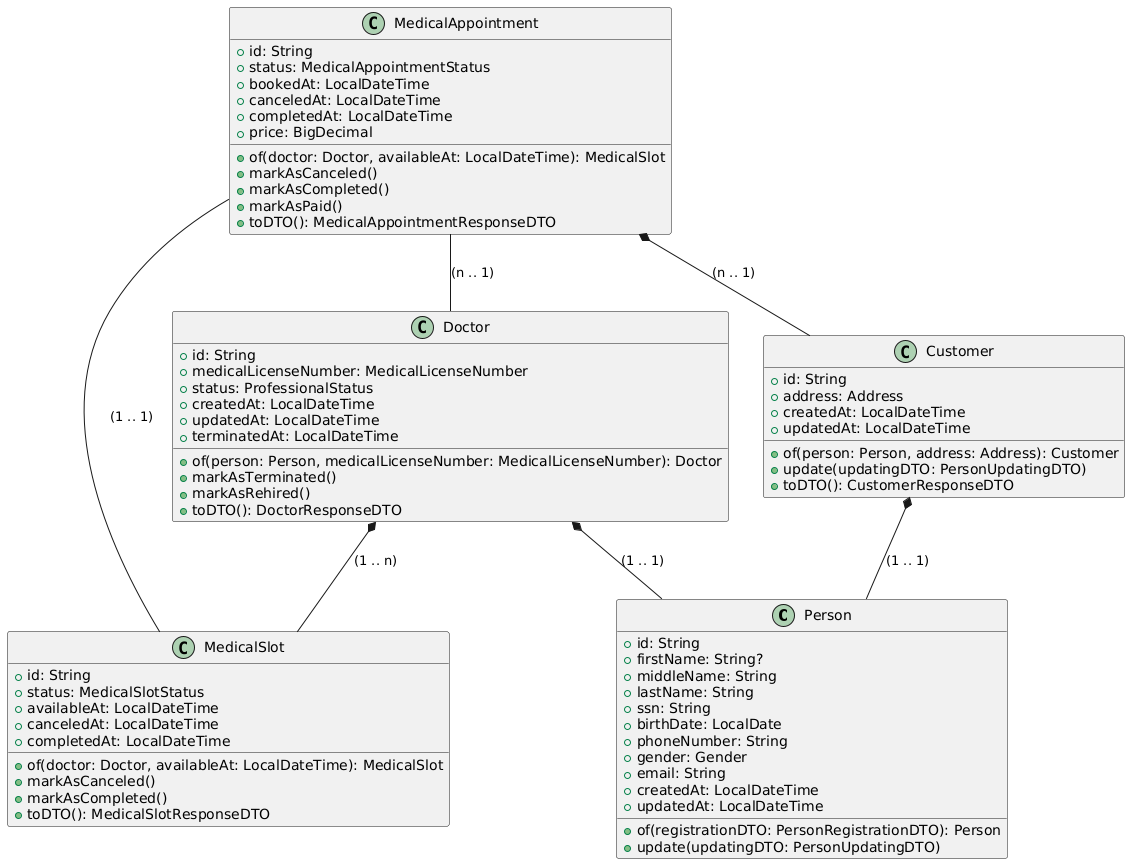
\includegraphics[width=1\linewidth]{figures/api/class_diagram.png}
    \label{fig:class_diagram}
    \\ \footnotesize Source: Author's creation
\end{figure}
\end{landscape}

From the \ref{fig:class_diagram}, it is notable that both \textbf{Customer} and \textbf{Doctor} have a one-to-one relationship with \textbf{Person}. One \textbf{Doctor} can be associated with multiple  \textbf{MedicalSlot} and 
\textbf{MedicalAppointment}, while \textbf{Customer} can be associated with multiple \textbf{MedicalSlot}. One \textbf{MedicalSlot} can associate with only one \textbf{MedicalAppontment}. One \textbf{Card} can be associated with multiple  \textbf{Payment}. It can be associated with only one \textbf{MedicalAppointment}.

Similar to the class diagram, the figure \ref{fig:class_diagram} displays the ERD. \cite{CAGILTAY20132184} agrees that the ERD provides an overall grasp of the data requirements, modeling, and database structures of the information system before the implementation phase. Therefore, as exposed by the figure \ref{fig:erd}, every model, except \textbf{Person} and
 \textbf{Card}, has at least one embedded model inside it, as listed below in the Table \ref{entity_relationships}:

\begin{table}[H]
\centering
\caption{Entity Composition Relationships}
\label{entity_relationships}
\begin{tabular}{p{0.4\textwidth}p{0.5\textwidth}}
\toprule
\textbf{Parent Entity} & \textbf{Contained Entities} \\
\midrule
Customer & Person \\ \hline
Doctor & Person \\ \hline
Payment & Card, MedicalAppointment \\ \hline
MedicalSlot & Doctor, MedicalAppointment \\ \hline
MedicalAppointment & Customer, Doctor \\
\bottomrule
\end{tabular}
\footnotesize Source: Author's creation.
\end{table}

The first major visual difference between the figure \ref{fig:class_diagram}, that embodies a class diagram, and the figure \ref{fig:erd}, that embodies an ERD, is that the ERD can contain embedded objects within its models. While class diagrams focus on static objects like models and the relationships among them, ERD focus on portraying the architecture of the system. 

Because ERDs can include embedded objects within their models, they serve as valuable managerial analysis tools. This capability allows the diagram to illustrate a more comprehensive view of the domain layer's models and their embedded objects within the API's architecture. By visualizing how each embedded object is integrated and interacts with its parent model and the overall system architecture, ERDs facilitate a deeper understanding of the system's design.

While the ERD's capacity to represent embedded objects offers a significant advantage in visualizing the system's architecture and the intricate relationships within its data structures, it is crucial to recognize that it complements, rather than replaces, the class diagram. Class diagrams excel at defining the static structure of the system, clearly outlining the classes, their attributes, methods, and the various types of relationships between them, such as inheritance, association, and aggregation. 

This provides a fundamental blueprint of the system's conceptual model. The ERD, on the other hand, builds upon this foundation by focusing on the data perspective, illustrating how entities are organized, their attributes, and the relationships crucial for data management and persistence. By showing how embedded objects are contained within these entities, the ERD offers a more granular view of the data's composition and flow within the system's architecture. Therefore, a comprehensive understanding necessitates the use of both diagrams. 

The class diagram provides the abstract, object-oriented view of the system's building blocks, while the ERD offers the concrete, data-centric perspective, detailing how these building blocks are instantiated and interconnected at the data level. This dual perspective allows for a more thorough analysis, ensuring that both the structural integrity of the system's objects and the efficient organization of its data are well-understood and effectively designed.

\begin{figure}[H]
    \caption{Entity-Relationship Diagram}
    \centering
    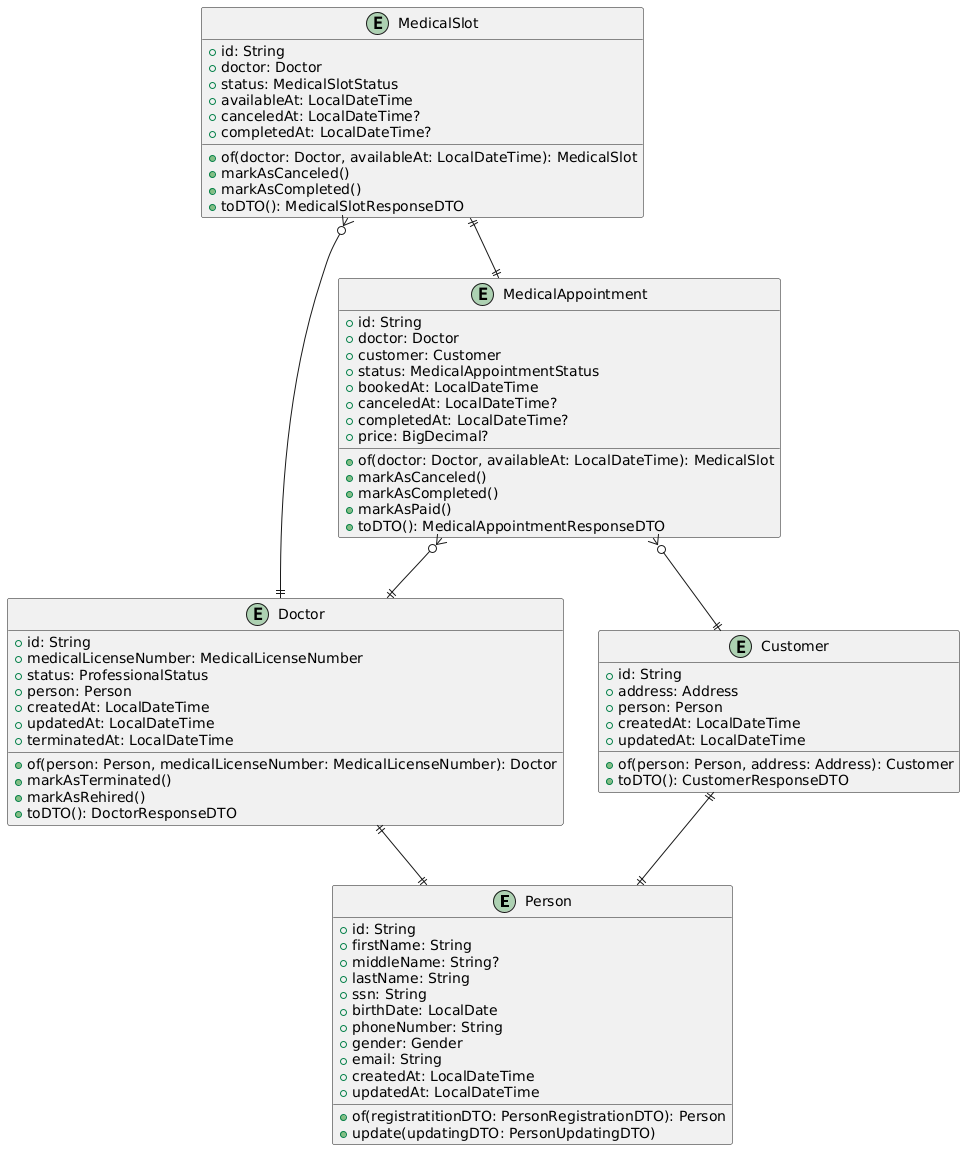
\includegraphics[width=1\linewidth]{figures/api/erd.png}
    \label{fig:erd}
    \\ \footnotesize Source: Author's creation
\end{figure}

Complementary to the aforementioned paragraph, it is notable the presence of embedded objects in the classes in the figure \ref{fig:erd}, which indicates that the adopted database is likely a NoSQL database, due to the presence of objects instead of any foreign keys, which the schema flexibility permits foreign keys to be used, as discussed in the \hyperref[subsection:database]{subsection MongoDB}.

Additionally, \cite{nanthaamornphong2019extended} cites that the class diagrams are the design from which other models are derived. For this reason, APIs's models are modeled according to the class diagram. The use of class diagrams comes with the actual reflection of real-world information, as evaluated by \cite{vo2020transformation}. 

Conceptually, a class of \hyperref[appendix:glossary]{UML} class diagram is, according to \cite{BERARDI200570, vo2020transformation}, a set of objects with 
common features whose attributes represent real-world data. In order to exemplify it, the figure \ref{fig:person_class} is the \hyperref[appendix:glossary]{UML} class diagram's class that represents statically the model \textbf{Person}. 

\begin{figure}[H]
    \caption{Example of a UML Class Diagram's Class}
    \centering
    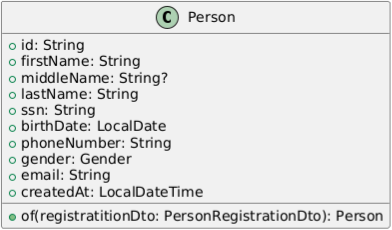
\includegraphics[width=0.87\linewidth]{figures/api/person_class.png}
    \label{fig:person_class}
    \\ \footnotesize Source: Author's creation
\end{figure}

As demonstrated by the figure \ref{fig:person_class}, the class was used to create the Java model presented in the figure \ref{fig:java_person_model}, that will be persisted into a MongoDB document. 

\begin{figure}[H]
	\centering
	\caption{Java Model of Person}
	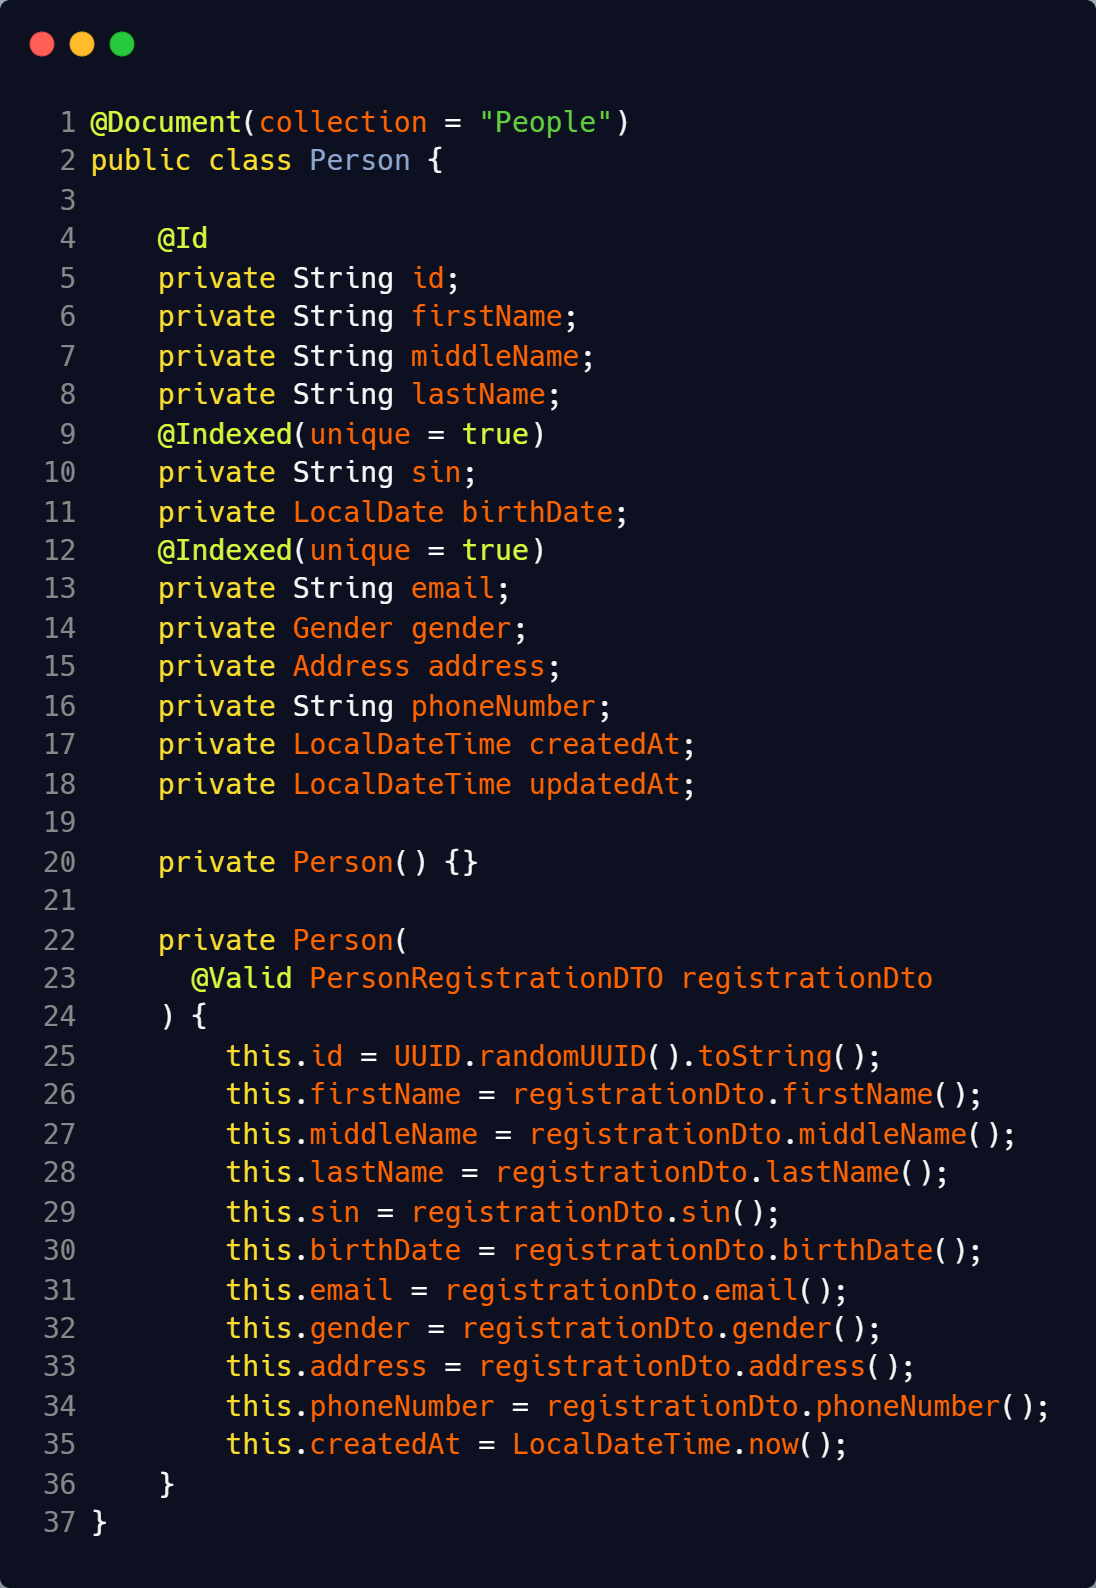
\includegraphics[width=1\linewidth]{figures/api/java_person_model.png}
	\label{fig:java_person_model}
	\footnotesize Source: Author's creation.
\end{figure}

The shift from the class diagram to a model was possible due to the precision of the modeling that the \hyperref[appendix:glossary]{UML} class diagram offers.

Moreover, the selected API for this work is the present in the \href{https://github.com/LazaroDamasceno/Reactive-Medical-Appointments-Management-API.git}{clickable link}, hereafter referred to as \textit{the API} which was developed by the author of this dissertation. It was developed using  \hyperref[appendix:glossary]{Spring Boot}, Java and WebFlux, and adopts reactive and non-blocking programming. Its domain models are defined in figure \ref{fig:class_diagram}, with their relationships illustrated in figure \ref{fig:erd}.

Formally, an API is a standardized set of tools, protocols, and definitions that enable interoperability—the ability of disparate systems to communicate seamlessly despite differences in language, platform, or interface. APIs provide both an abstraction layer for system interactions and concrete implementations (e.g., packaged classes or interface types). As controlled data-sharing mechanisms, they facilitate resource reuse and multi-source integration, addressing critical needs in application development 
 and research 
 \cite{aksu2016visualization, dullabh2020application, hussain2020enterprise, matilainen2011multicore, mcguire2013publisher, 
 swaminathan2016review, wegner1996}.

Additionally to the aforementioned paragraph, the API adopts the modular monolith instead of microservices or monolith architectures. 
\cite{su2024modular} defines modular monolith as an architecture that blends the simplicity of a monolith with the benefits of microservices. The author too informs that it structures the system into loosely coupled modules with clear boundaries and explicit dependencies. Each module remains independent and isolated, enabling separate development while being deployed as a single unit.

This approach strikes a middle ground between monoliths and microservices, emphasizing interchangeability, reusability, and well-defined interfaces. It simplifies development, testing, and deployment by encapsulating functionality within modules \cite{su2024modular}.

An example is Spring Modulith, an experimental Spring project that enforces modularity in Spring Boot applications. It provides conventions for declaring and validating modules, ensuring proper encapsulation and controlled exposure of Spring Beans. Modules can be organized as sub-packages, with restricted visibility between them to maintain clean boundaries \cite{su2024modular}.

Considering the explanation of Spring Modulith, the API uses Spring Modulith to organize its files. The project permits hiding components such as controllers, implementation classes of the services, repositories, and permits the exposure of components such as exceptions, utility classes, extension functions, and interfaces of the services. 

One example is: the module \textit{people} has as sub-module \textit{services}, that has as files the interface 
\textit{PersonRegistrationService}, which is an interface, as illustrated in the figure \ref{fig:person_registration_service}. The class \textit{PersonRegistrationServiceImpl}, which is the implementation of an interface, is illustrated in the figure \ref{fig:person_registration_service_impl}. Hereafter, both figures shall be referred to, respectively, as \textit{the interface} and \textit{the implementation} for brevity.

\begin{figure}[H]
    \centering
    \caption{Person Registration Service}
     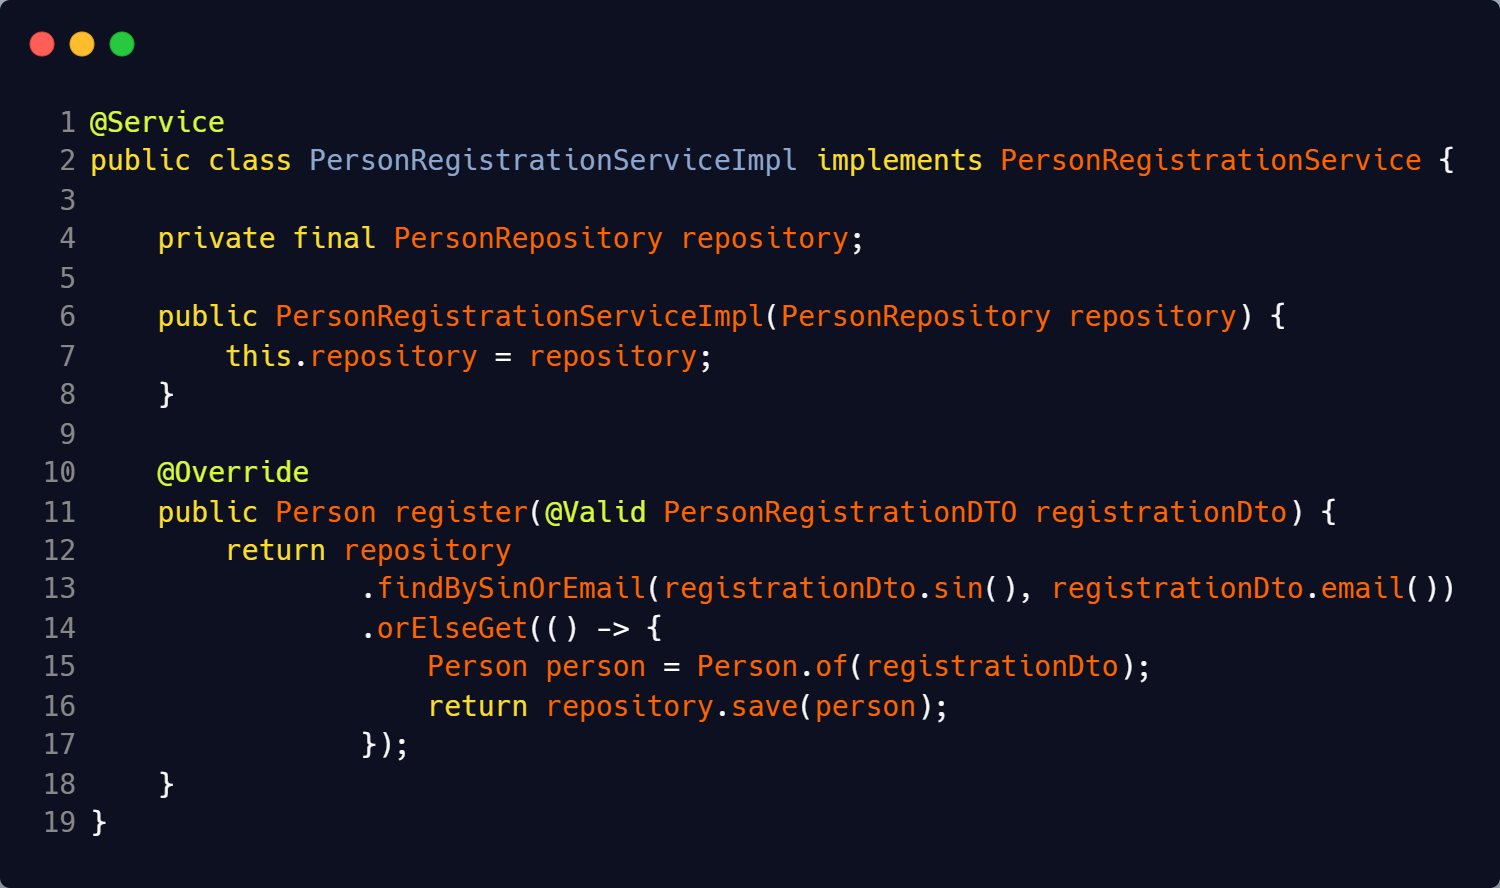
\includegraphics[width=1\linewidth]{figures/http/person_registration_service.png}
    \label{fig:person_registration_service}
    \footnotesize Source: Author's creation
\end{figure}

\begin{figure}[H]
    \centering
    \caption{Person Registration Service Implementation}
    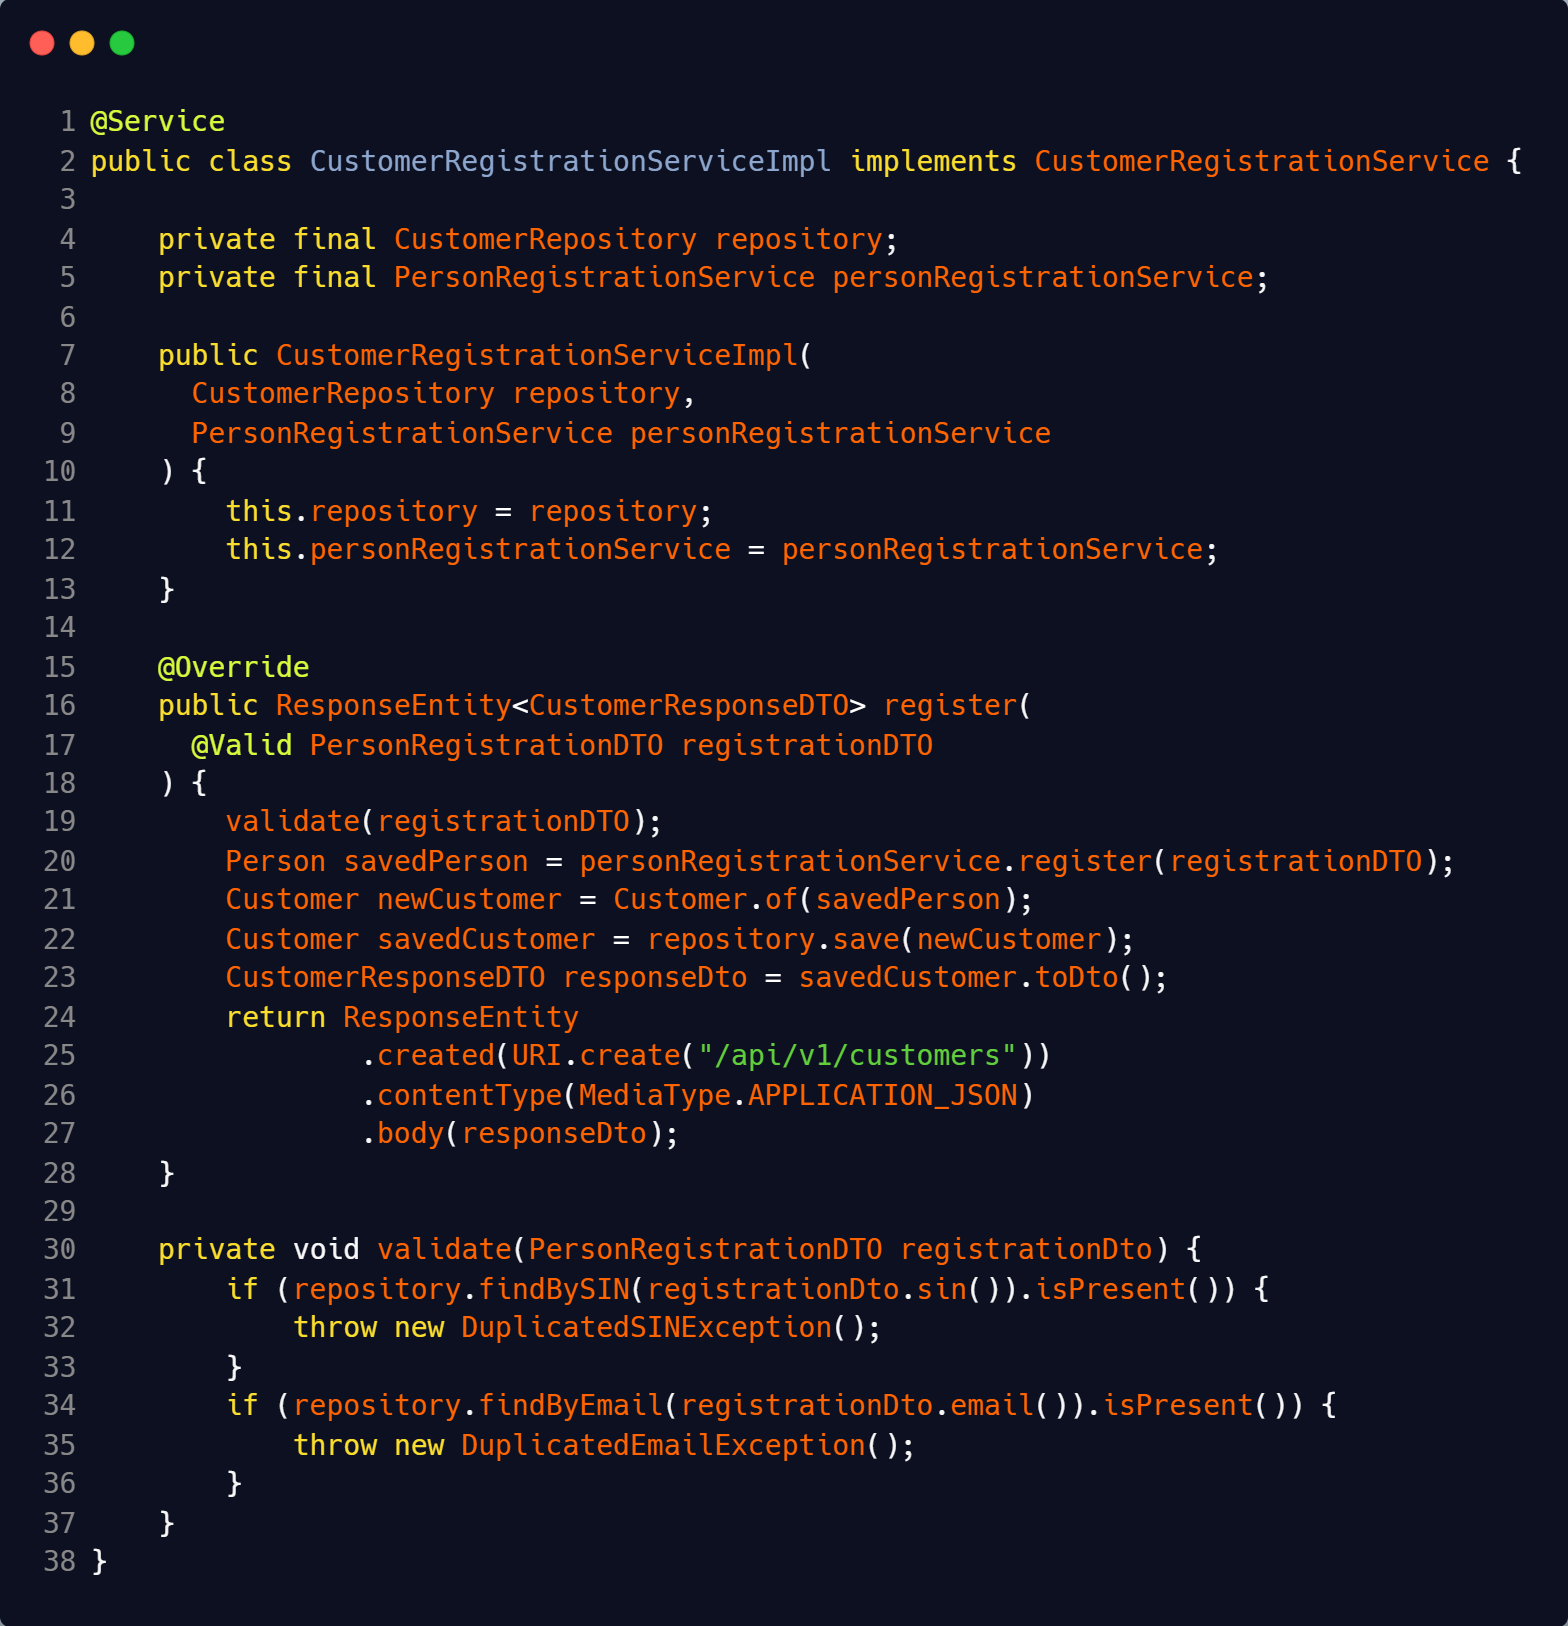
\includegraphics[width=0.87\linewidth]{figures/http/customer_registration_service_impl.png}
    \label{fig:person_registration_service_impl}
    \\ \footnotesize Source: Author's creation
\end{figure}

The implementation includes a repository (\textit{personRepository}), shown in figure \ref{fig:person_registration_service_impl}. 
As the repository acts as an abstraction between layers—specifically within the data access layer—it manages database operations according to \cite{prajapati2019asp}. Since repositories handle sensitive data, they must be restricted from unrelated components to prevent unauthorized or 
unintended access. This is achieved through the interface depicted in figure \ref{fig:person_registration_service}, which abstracts the implementation and enforces access control.

In summary, the API is responsible for the tasks listed in the Table \ref{api_functionalities_grouped}:

\begin{table}[H]
\centering
\caption{API Functionalities by Domain}
\label{api_functionalities_grouped}
\begin{tabular}{p{0.3\textwidth}p{0.6\textwidth}}
\toprule
\textbf{Domain} & \textbf{Functionalities} \\
\midrule
Person Management & Customer registration, Doctor registration/termination/rehiring \\ \hline
Medical Slots & Registration, cancellation, completion \\ \hline
Medical Appointments & Registration, cancellation, completion \\ \hline
Data Operations & Retrieval \\ \hline
Payment Simulation & Card creation, appointment payment \\
\bottomrule
\end{tabular}
\footnotesize Source: Author's creation.
\end{table}

The functionalities listed in the Table 
\ref{api_functionalities_grouped} represent the core tasks performed by the API's service layer. These operations are visualized in the component diagram (figure \ref{fig:component_diagram}), which—as noted by \cite{rajagopal2017study}—portrays the API's component organization. \cite{bell2003uml, rajput2015uml} cite that A \hyperref[appendix:glossary]{UML} component diagram shows the physical structure of a system, illustrating software components (e.g., libraries, executables) and their dependencies. It focuses on the system's modular building blocks, not functionality, and can be viewed at different levels of detail. Multiple component diagrams are needed for complex systems, providing insights into implementation, dependencies, and modularity, aiding system construction.

\begin{landscape}
\begin{figure}[H]
    \centering
    \caption{Component Diagram}
    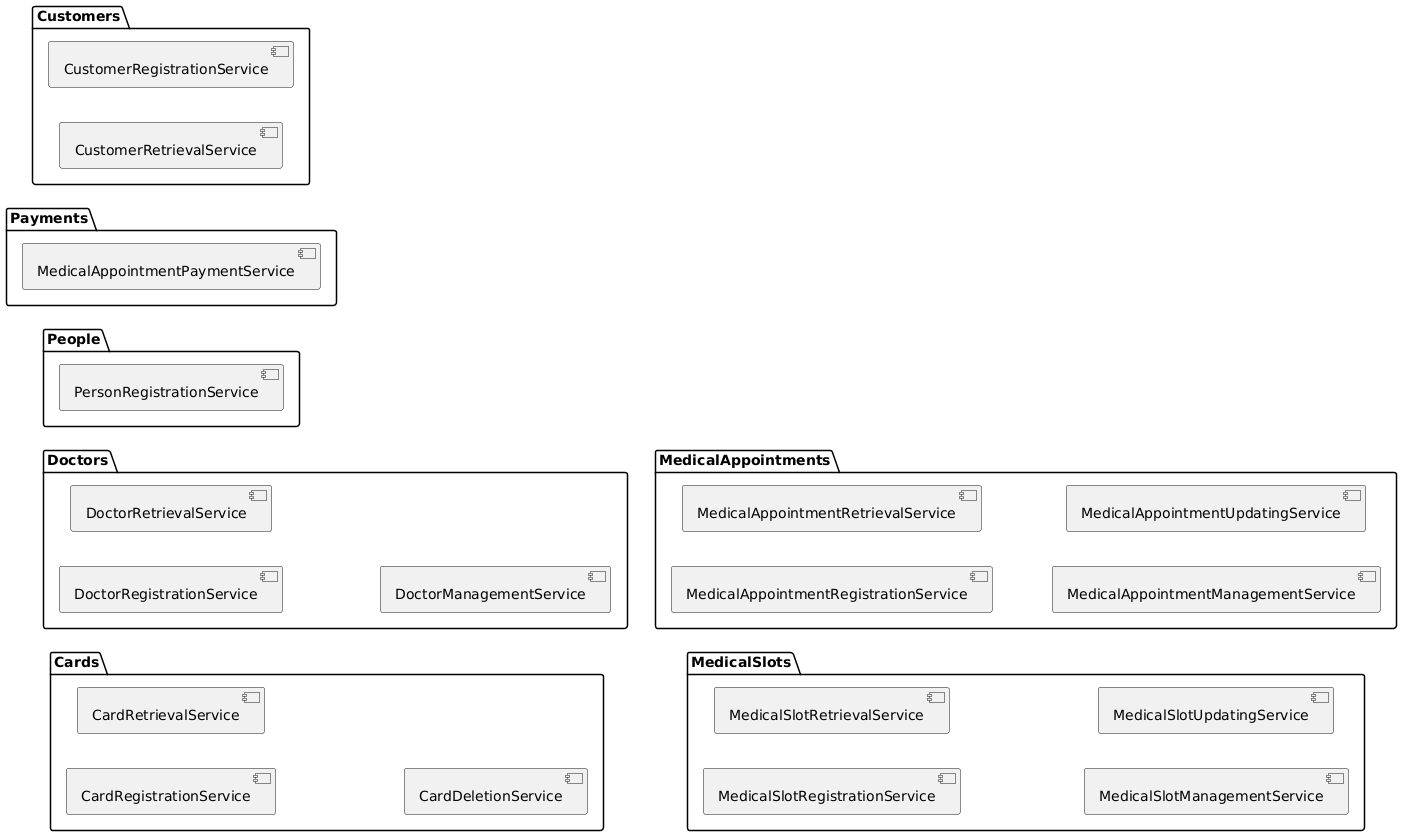
\includegraphics[width=0.99\linewidth]{figures/component_diagram.png}
    \label{fig:component_diagram}
    \\ \footnotesize Source: Author's creation
\end{figure}
\end{landscape}

The organization of the API is divided into 7 different modules and 18 services, although not all services were selected to undergo the planned software tests. The selected services are shown in the Table \ref{tab:selected_services}:

\begin{table}[H]
	\centering
	\caption{API's Selected Services}
	\label{tab:selected_services}
	\begin{tabular}{ll}
		\textbf{Modules} & \textbf{Services} \\ \hline
		payments & MedicalAppointmentPaymentService \\ \hline
		doctors & DoctorRegistrationService, DoctorUpdatingService, \\
		& DoctorManagementService \\ \hline
		customers & CustomerRegistrationService, CustomerUpdatingService \\ \hline
		medicalAppointments & MedicalAppointmentManagementService, \\
		& MedicalAppointmentRegistrationService \\ \hline
		medicalSlots & MedicalSlotManagementService, MedicalSlotRegistrationService \\ \hline
	\end{tabular}
	\\ \footnotesize Source: Author's creation.
\end{table}

From the API's services, 10 out of 18 were selected. The test coverage is 55,56\%. Additionally, the excluded services are:

\begin{enumerate}
    \item PersonRegistrationService.
    \item CustomerRetrievalService.
    \item DoctorRetrievalService.
    \item CardRetrievalService.
    \item CardRegistrationService.
    \item CardDeletionService.
    \item MedicalAppointmentRetrievalService.
    \item MedicalAppointmentUpdatingService.
    \item MedicalSlotRetrievalService.
    \item MedicalSlotUpdatingService.
\end{enumerate}

These services were not selected primarily because their responses generally do not require a validation process to verify expected wrongful conditions and the subsequent throwing of exceptions. Furthermore, even in the cases where these services might throw an exception, it is not considered sufficiently important to include them in the unit and integration tests.

The selected services are the most essential and important of the API. They represent the most used functions. They are the core of the application.

Finally, the endpoints of the API are shown in the figures \ref{fig:swagger_ui_1}, \ref{fig:swagger_ui_2}, and \ref{fig:swagger_ui_3} 
displaying the \hyperref[appendix:glossary]{user interface} that Swagger UI generated for the API's endpoints.


\begin{figure}[H]
	\centering
	\caption{Swagger UI - Page 1}
	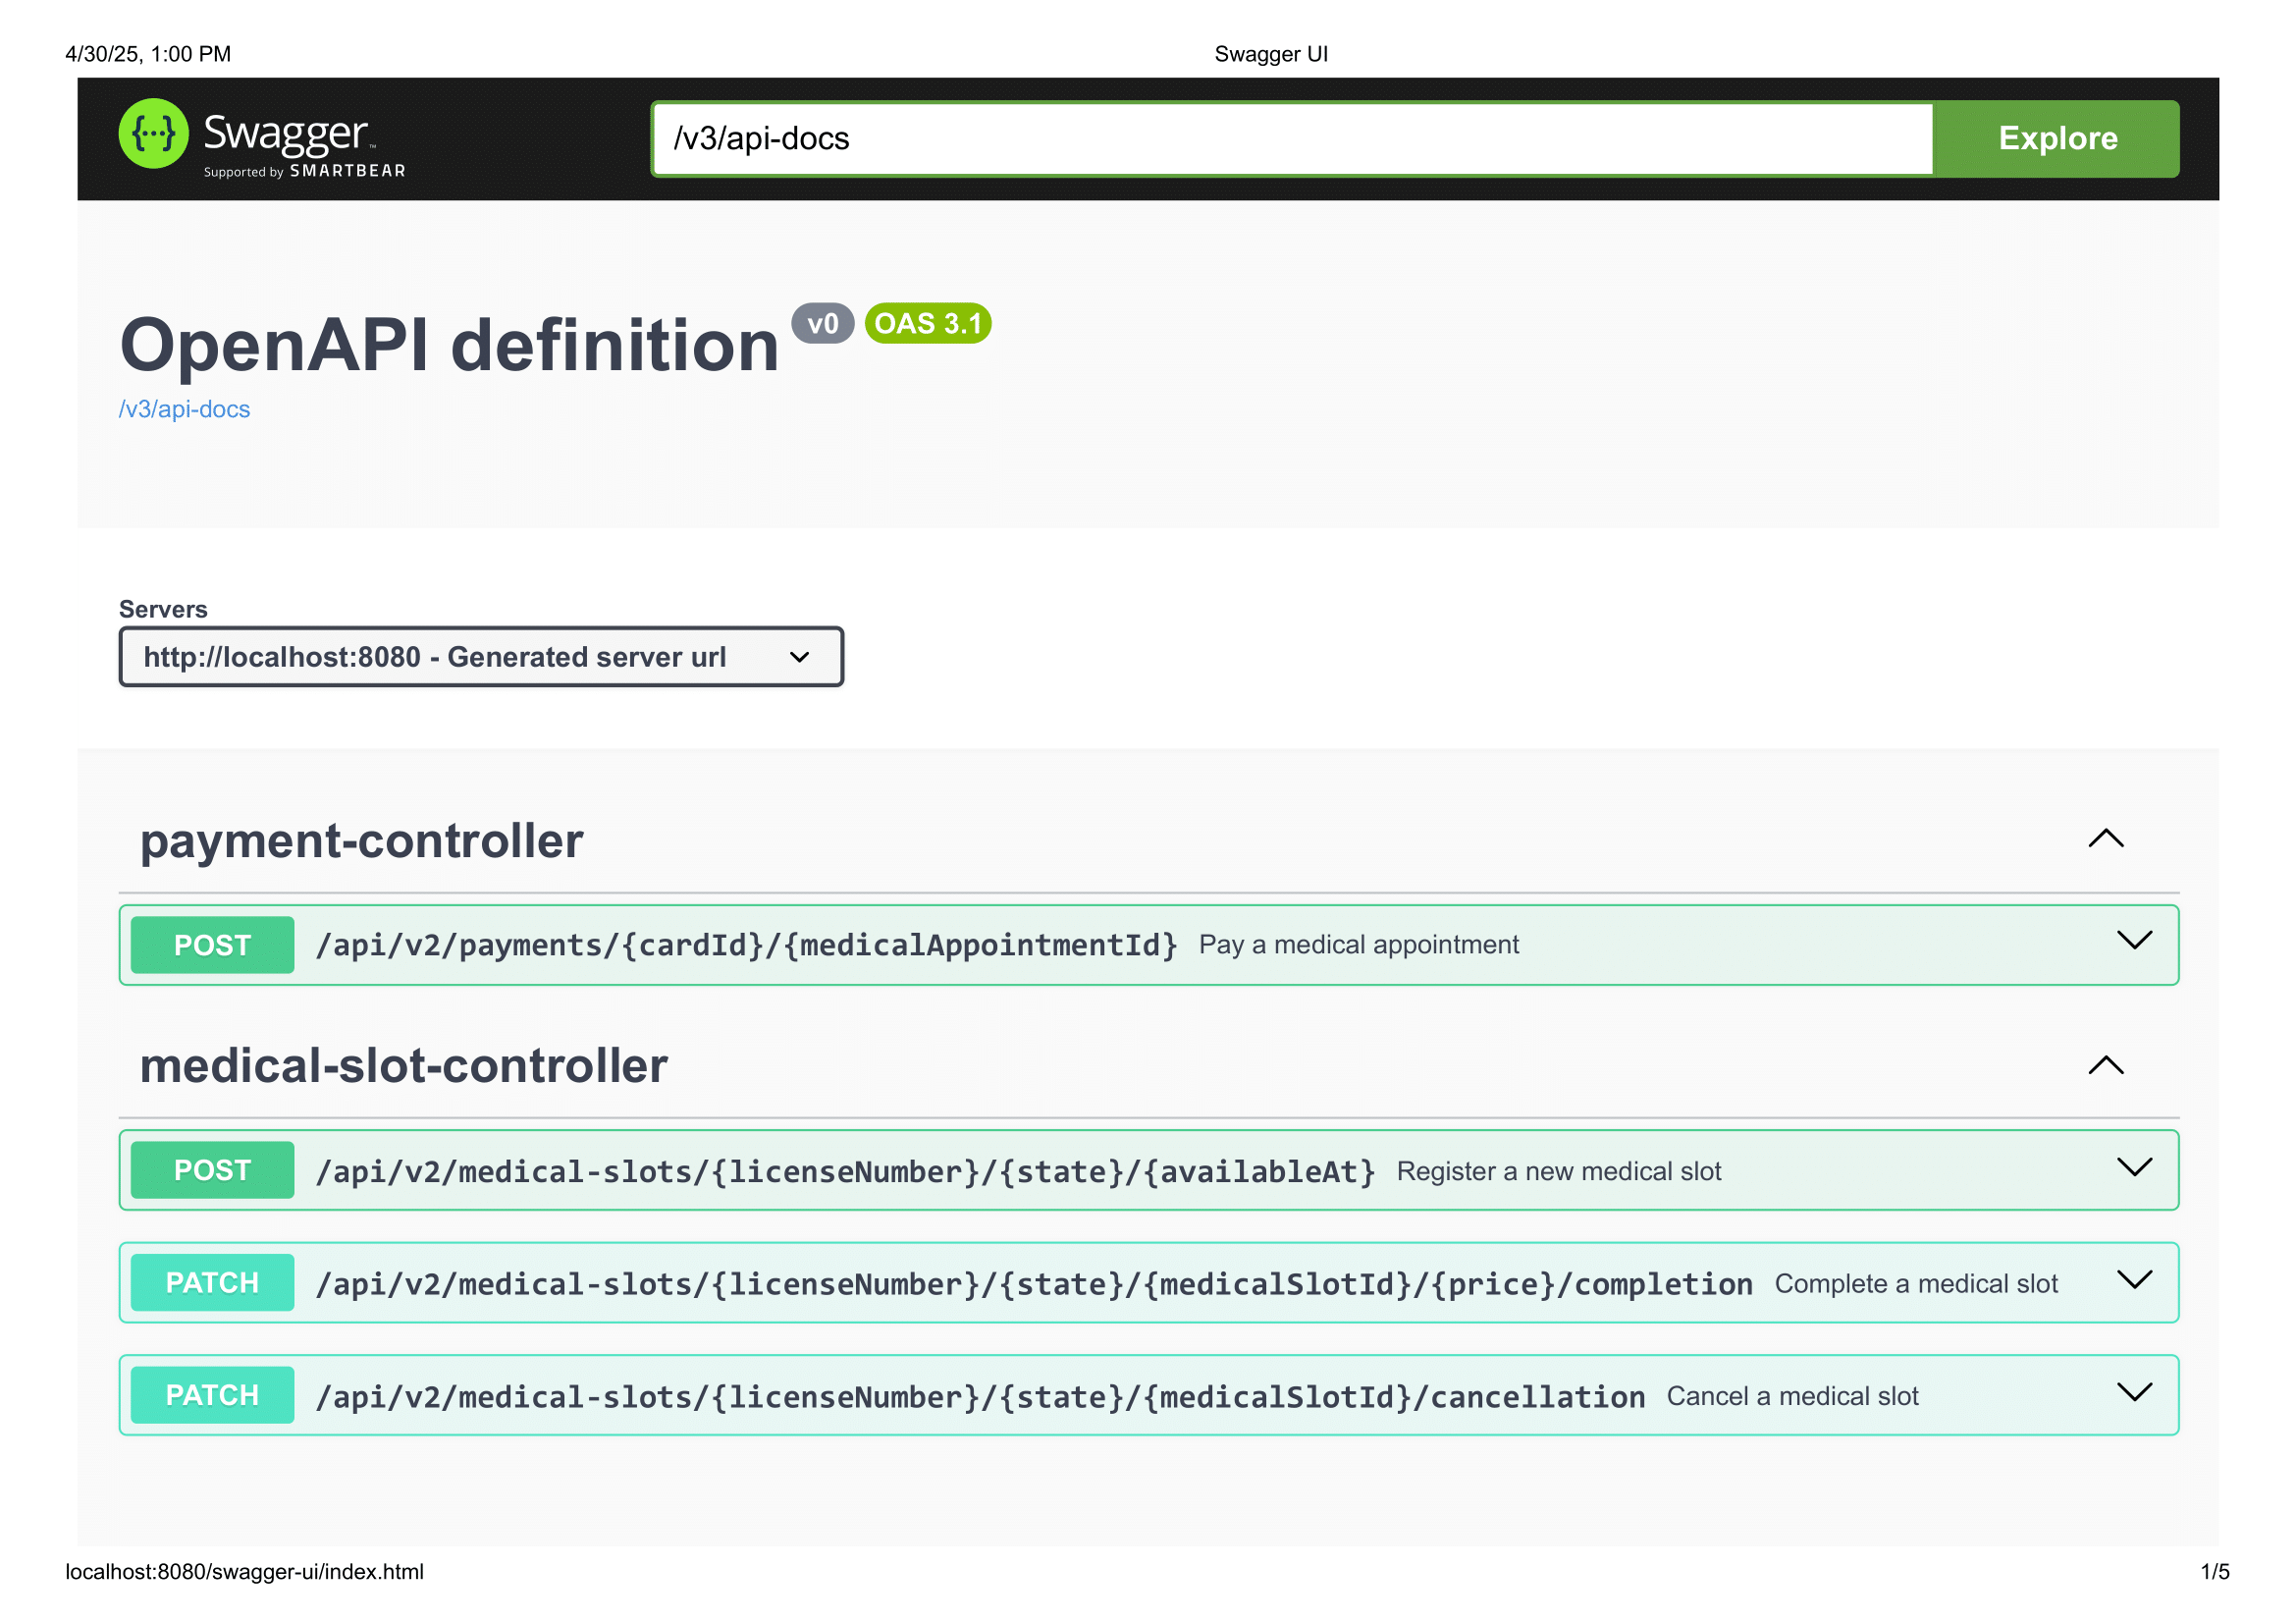
\includegraphics[width=0.83\linewidth]{figures/swagger_ui_1.png}
	\label{fig:swagger_ui_1}
	\\ \footnotesize Source: Author's creation.
\end{figure}

\begin{figure}[H]
	\centering
	\caption{Swagger UI - Page 2}
	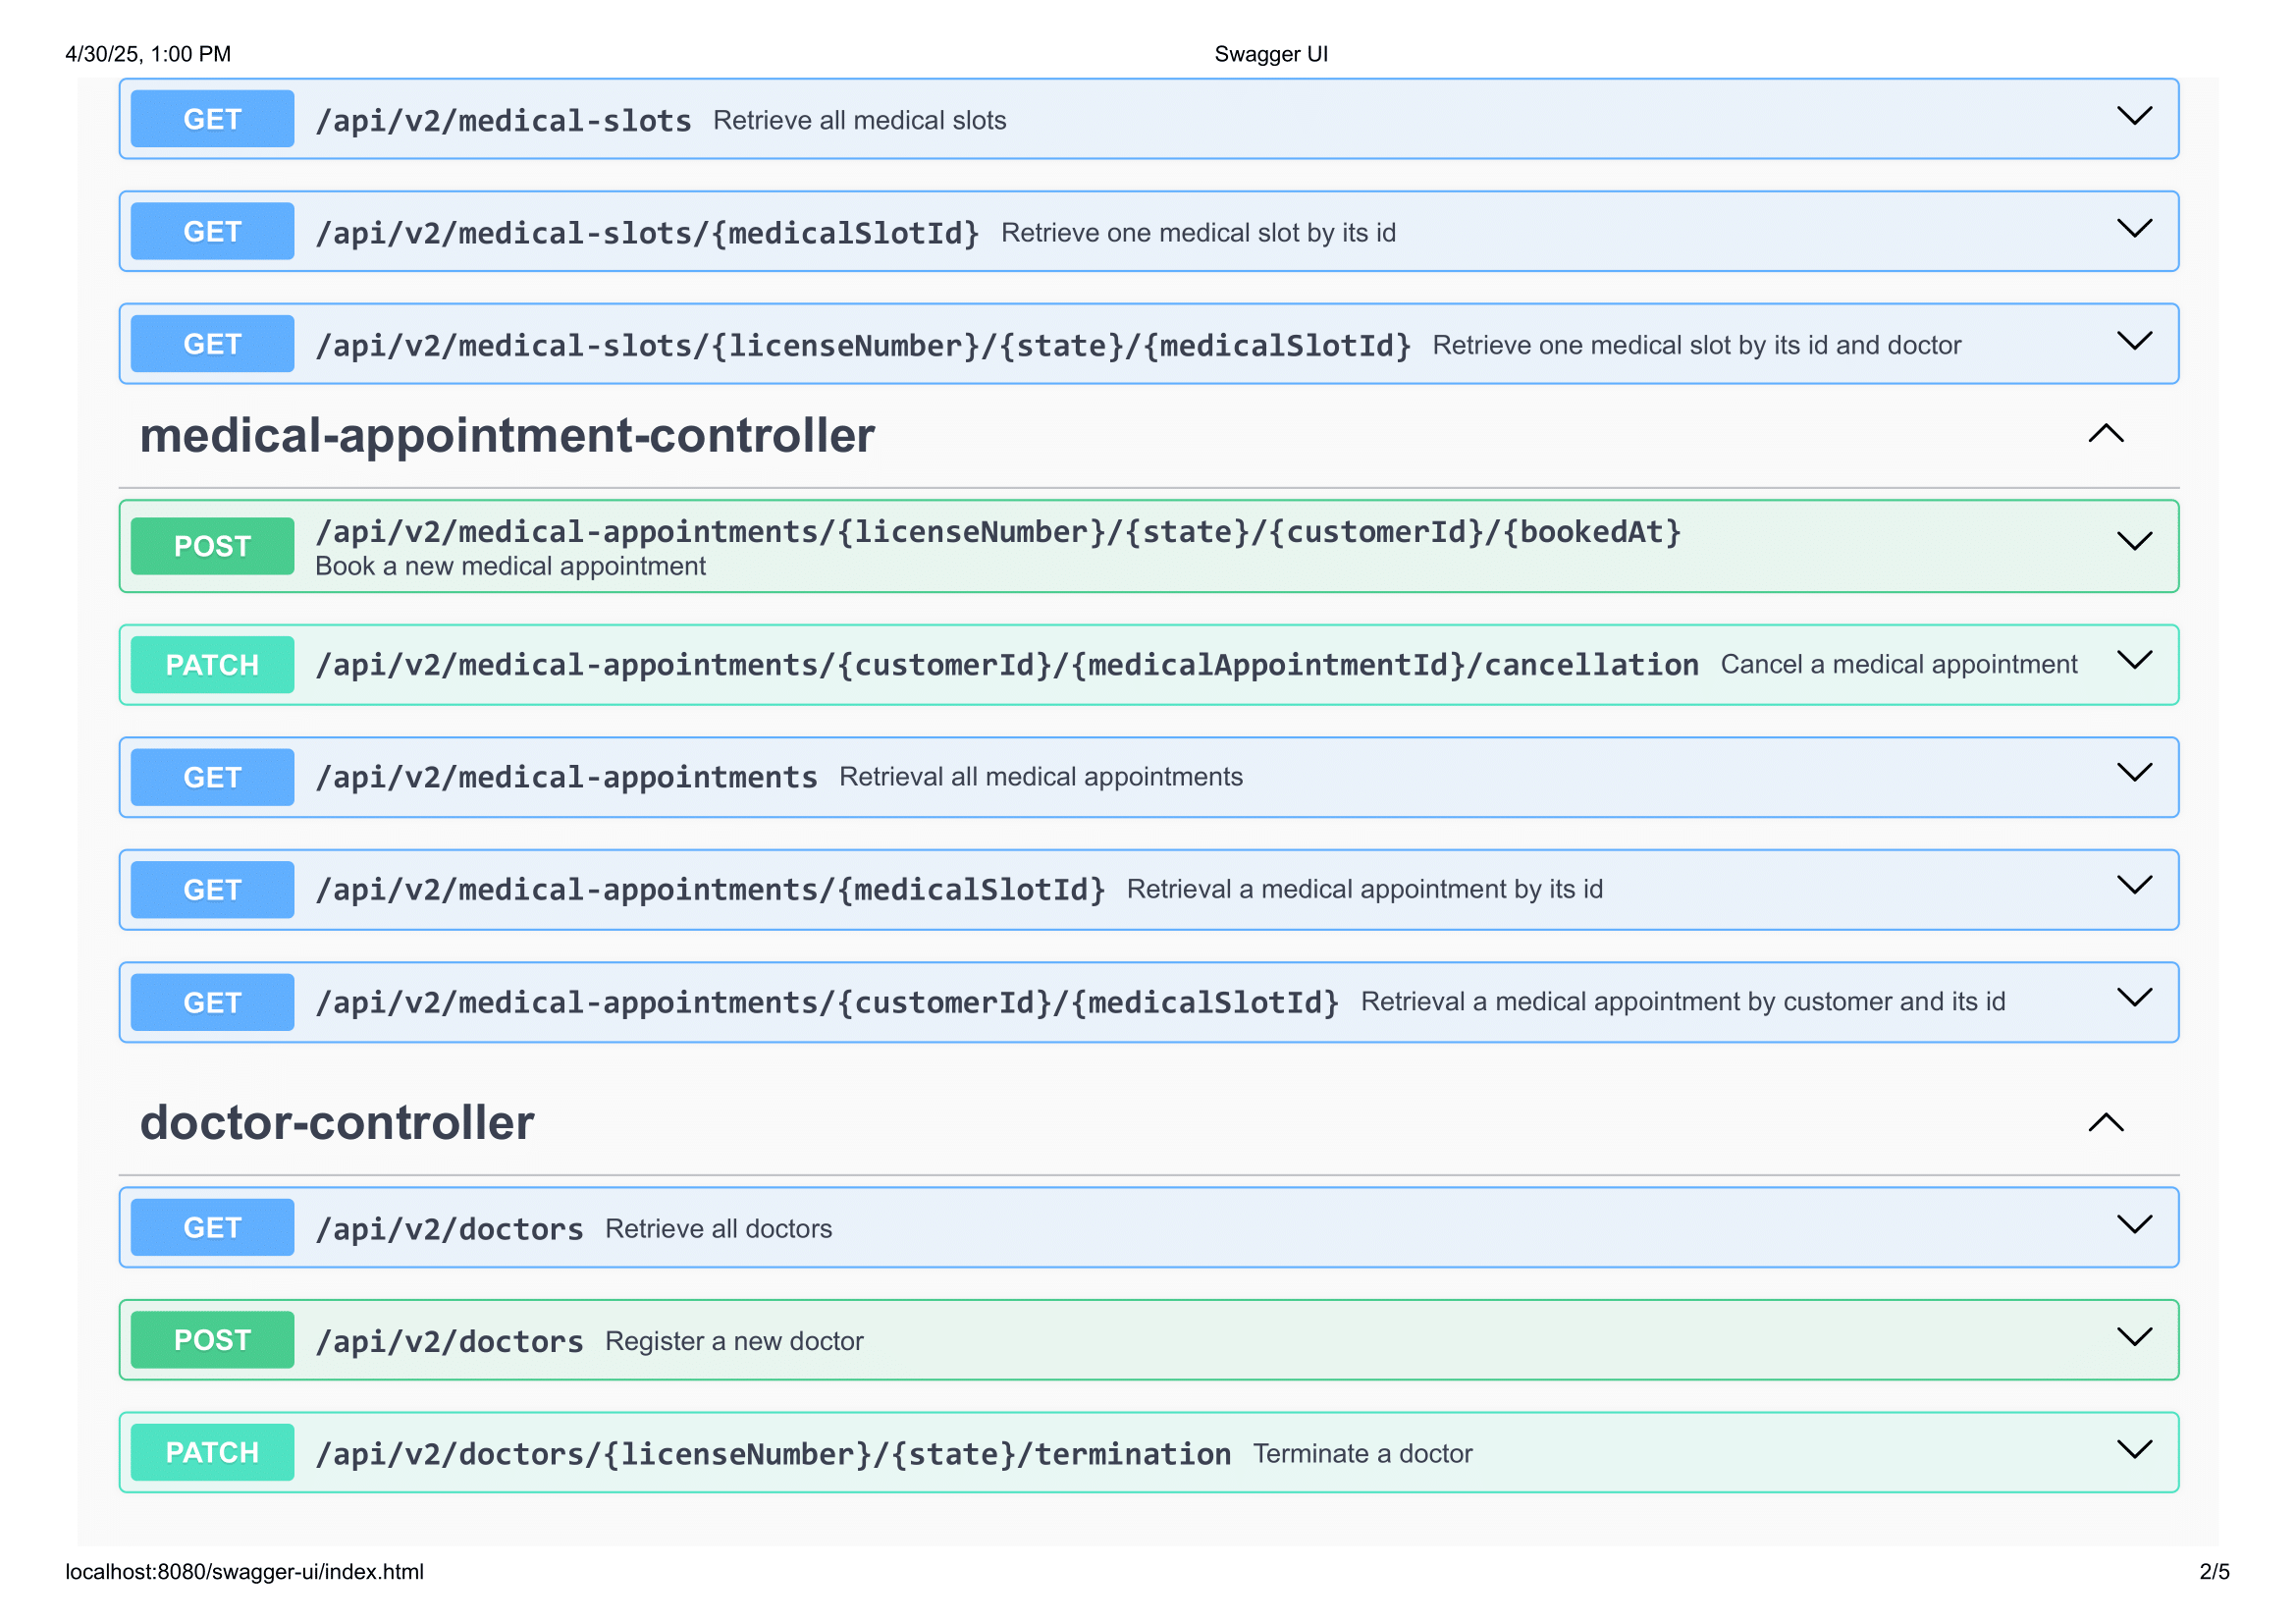
\includegraphics[width=0.83\linewidth]{figures/swagger_ui_2.png}
	\label{fig:swagger_ui_2}
	\\ \footnotesize Source: Author's creation.
\end{figure}

\begin{figure}[H]
	\centering
		\caption{Swagger UI - Page 3}
		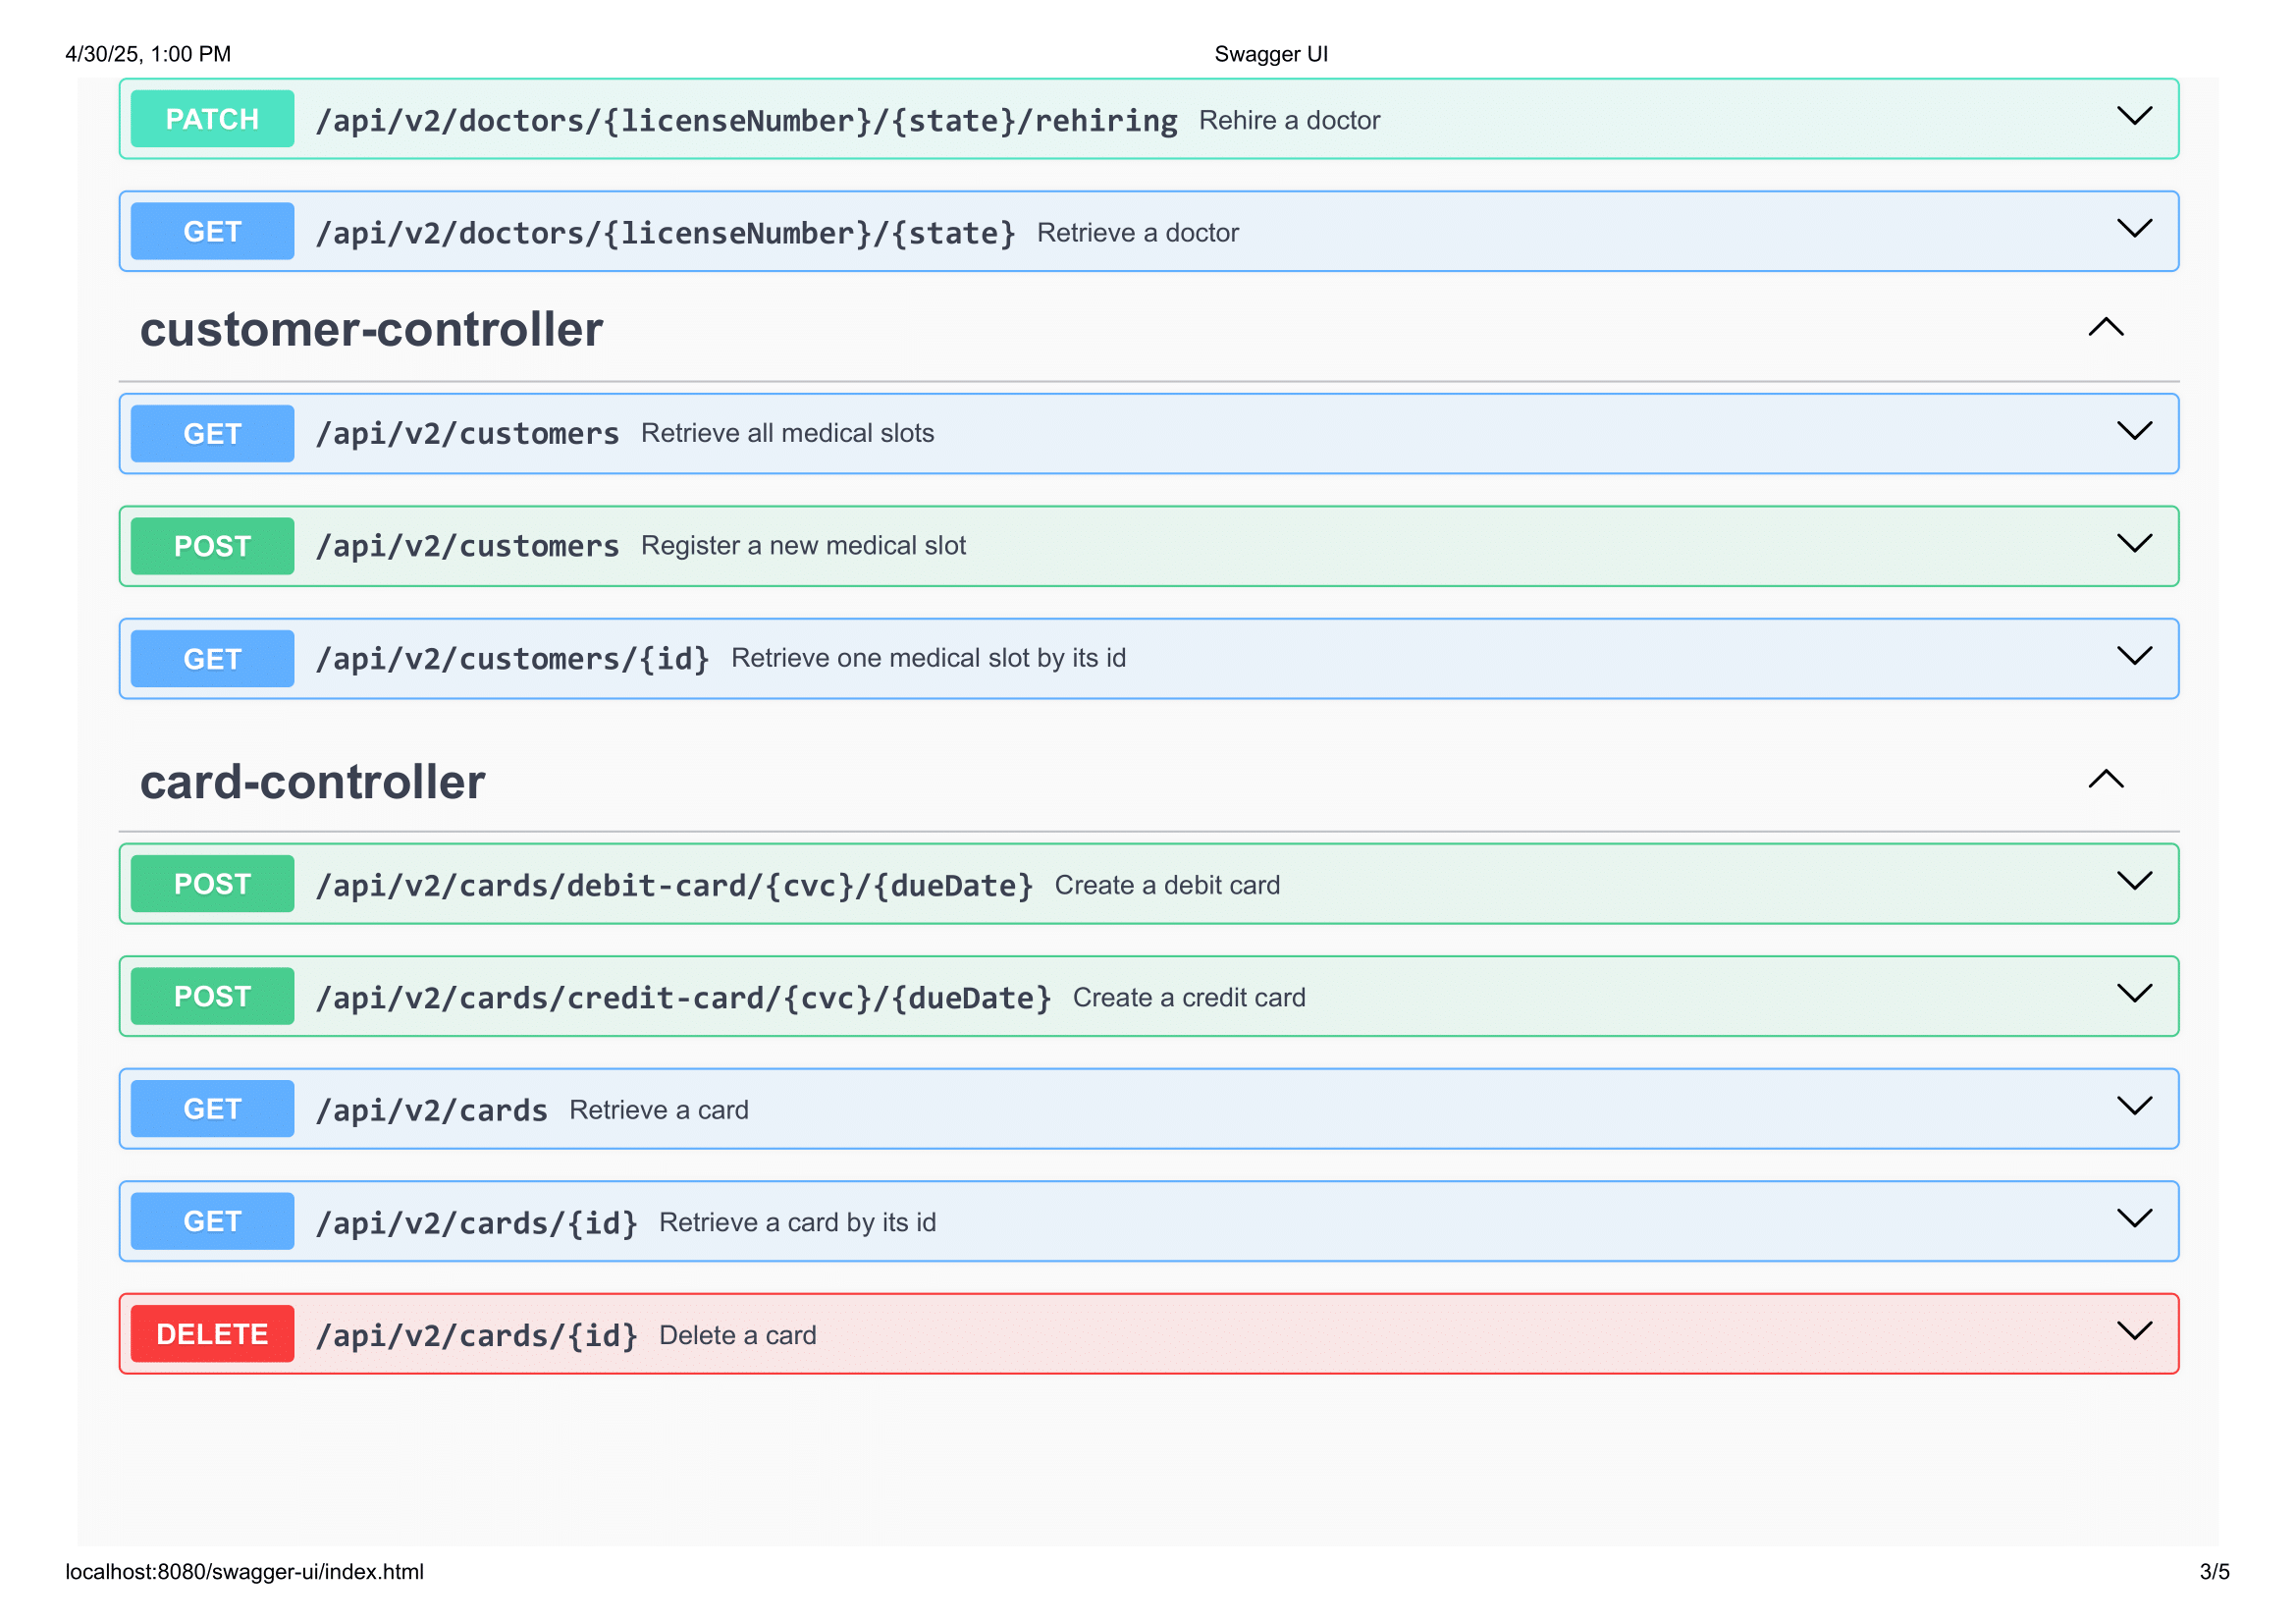
\includegraphics[width=0.83\linewidth]{figures/swagger_ui_3.png}
		\label{fig:swagger_ui_3}
		\\ \footnotesize Source: Author's creation.
\end{figure}

As discussed by the \hyperref[subsection:http_semantics]{subsection HTTP Semantics}, the endpoints present in the figures \ref{fig:swagger_ui_1}, 
\ref{fig:swagger_ui_2}, and \ref{fig:swagger_ui_3} are compliant with \hyperref[appendix:glossary]{RFC} \href{https://www.rfc-editor.org/rfc/rfc9110.html}{9110} in both methods's guidelines and \hyperref[appendix:glossary]{URI} format, due to the presence of the method and the \hyperref[appendix:glossary]{URI}'s relative path. Swagger UI was used to create the content shown in the figures \ref{fig:swagger_ui_1}, \ref{fig:swagger_ui_2}, and \ref{fig:swagger_ui_3}, due to its ability, as stated by \cite{mcnamara2022flexible}, to expose graphically API resources, which are automatically generated from an OpenAPI Specification.\footnote{\href{https://swagger.io/tools/swagger-ui/}{See the official site of Swagger UI.}}

\subsection{Automated Software Testing}
\label{subsection:automated_software_testing}

Testing, one of the most crucial tasks along the \hyperref[appendix:glossary]{SDLC}, can easily exceed half of a project’s total effort. A successful testing approach can save significant effort and increase product quality, thereby increasing customer satisfaction and lowering maintenance costs \cite{juristo2006guest, tuteja2012research}

The potentially vast scope of testing can be visualized as sticking small pins into a doll, representing limited coverage across a large domain. This analogy underscores the necessity of maintaining a realistic expectation of 
what testing can achieve. Consequently, while capable of identifying various errors and bugs, the inherent limitations mean that not all defects may be discovered, and thus the importance of testing should not be overemphasized. 
Recognizing that different testing techniques are complementary, a comprehensive approach utilizing multiple methods offers the greatest likelihood of detecting the majority of errors 
\cite{meyer2008seven, pocatilu2002automated, sethi2017review, yadav2019software}.

In contrast with the previous paragraph, testing is an indispensable approach that improves the quality of the system as well as increases the chances of a successful effort. Additionally, it is required to remove the discrepancy in the development process of the software product development \cite{jindal2016importance}.

Furthermore, testing is defined by \cite{huang2003automated} as the standard process used to validate that software conforms to the formal requirements. \cite{vijayasree2022review} is the process of writing a program in any programming or scripting language that duplicates the manual test case steps with the help of an external automation helper tool. 

Good Testing implies more than just executing a program with desired inputs and expected output. Testing provides the chance to review requirements for important quality attributes. And it requires the planning of test cases, design of test cases, execution of test cases, and test review, which is given as feedback to the planning team. The dangerousness of the absence of tests in software tends to lead to more reckless use of resources and money, which is comparable to driving a car without any brakes or gears \cite{madhavi2016white}.

As  a consequence, before implementing any software product, tests must be made. They must follow a set of various phases. Testing activities ask questions and resolve issues earlier. There are many activities that are performed during the testing. According to \cite{jindal2016importance,pocatilu2002automated}, the testing process has the following activities: planning, design and implementation, execution, evaluation.

Software testing includes all activities aimed at identifying the differences between specifications of the software and the actual behavior.  The objectives of testing are the ones mentioned in the table \ref{tests_goals} 
\cite{anand2019importance, huang2003automated, hussain2015comparative}:

\begin{longtable}{p{0.25\linewidth}p{0.65\linewidth}}
    \caption{Key Aspects of Software Testing}
    \label{tests_goals} \\
    \toprule
    \textbf{Aspect} & \textbf{Description} \\
    \midrule
    \endfirsthead
    
    \multicolumn{2}{c}{\bfseries \tablename\ \thetable{} -- continued from previous page} \\
    \toprule
    \textbf{Aspect} & \textbf{Description} \\
    \midrule
    \endhead
    
    \midrule
    \multicolumn{2}{r}{Continued on next page} \\
    \endfoot
    
    \bottomrule
    \multicolumn{2}{c}{\footnotesize Resource: Adapated from \cite{anand2019importance, huang2003automated, hussain2015comparative}} \\
    \endlastfoot  

    Evaluation & Assesses works under uncommon conditions and demonstrates that components are prepared for integration. \\ \addlinespace \hline
    Revealing & Finds defects, errors, and deficiencies. Evaluates system capabilities and limitations, quality of components, work artifacts, and the system. \\ \addlinespace \hline
    Anticipation & Provides information to prevent or reduce errors, clarify 
    system specifications and execution. Identifies approaches to avoid
     risks and issues in the future. \\ \addlinespace \hline
    Improving quality & Effective testing minimizes errors and consequently  
    enhances software quality. \\ \addlinespace \hline
    Finding and Preventing Defects & The primary task is to identify defects and report 
    them for rectification. Testing reveals the presence of defects. \\ \addlinespace \hline
    Satisfying Requirements & Verifies compliance with Software Requirement Specification 
    and Business Requirement Specification to ensure user needs are met. \\ \addlinespace \hline
    Writing Quality Test Cases & Well-designed test cases validate requirements 
    and can uncover problems in requirements or application design. \\ \addlinespace \hline
    Reliability Estimation & Estimates the probability of failure-free operation
     and identifies the main failure causes. \\ \addlinespace \hline
    Time Management & Requires effective scheduling to achieve testing objectives 
    while ensuring timely delivery through early testing in each SDLC phase. \\ \addlinespace \hline
    Quality Orientation & Focuses on user perspective and continuous quality 
    improvement through proper quality attributes. \\ \addlinespace \hline
    Tester Traits & Includes creativity, innovative thinking, a positive attitude, intellectual curiosity, and quick learning ability. \\ 
\end{longtable}

Thereby, \cite{thant2023impact} argues that there are two types of software tests: manual and automated. The automated test is a type of software testing that uses software tools to execute test cases automatically. It 
involves the use of specialized testing software to perform the testing tasks instead of manual effort, while the manual test is a type of software 
testing that is carried out manually by a human tester. It involves the tester manually executing test cases without the use of automation testing tools.

Among the software testing, the automated testing, as cited by
\cite{khaliq2022artificial, pocatilu2002automated}, automated testing tools relieve the tester from the burden of the execution of the test cases, consist of a series of processes, activities, and tools that execute the software under test and record the results of the tests.

In addition, as  conveys, a potential testing tool should be capable of 
exercising as many program statements as possible on execution when given a program statement with a set of input parameters. As understandability, portability, and maintainability of executable test descriptions are necessary qualities, repeatability and accuracy are sought by testing users. This is one reason organizations are both to uncover bugs and ensure 
that they meet performance standards \cite{abo2023role}. 

Conversely, software test automation improves software quality and reduces software development costs in the long term by increasing the Return on Investment and further maturity of automatic test generation and debugging based on experience. Automation is not a quick solution for projects that are running behind schedule or over budget. There is a significant investment required to implement automated testing, but it is cost-effective when testing is performed on a regular basis. Software automation testing
 tools provide greater efficiency and consistency to the testing process, and have proven beneficial in terms of increasing quality while minimizing project schedules and effort \cite{abo2023role, huang2003automated}.

The types of tests are unit, integration, functional, system, acceptance, beta, and regression, as evidenced by \cite{meenakshi2014software}. The author describes in the table \ref{tab:general_description_of_tests} via a visual approach what the types of tests relate to their specifications, scopes, opacity, and responsible developers.

\begin{table}[htbp]
    \caption{General Description of the Types of Test}
    \label{tab:general_description_of_tests}
    \centering
    \setlength{\tabcolsep}{4.5pt} % Balanced padding
    \begin{tabular}{ *{5}{p{0.18\linewidth}} }
        \toprule
        \textbf{Testing Type} & \textbf{Specification} & \textbf{Scope} & \textbf{Opacity} & \textbf{Performed By} \\
        \midrule
        Unit & Low-level code design & Classes & White box & Programmer \\ \hline
        Integration & Multi-level design & Multiple classes & White/Black box & Programmer \\ \hline
        Functional & High-level design & Whole product & Black box & Testers \\ \hline
        System & Requirements & Product + environment & Black box & Testers \\ \hline
        Acceptance & Requirements & Product + environment & Black box & Customer \\\hline
        Regression & Code changes & Product + environment & White/Black box & Testers/Programmer \\
        \bottomrule
    \end{tabular}
    \vspace{-0.5em} % Tighten space below table
    \footnotesize Source: Adapted from \cite{meenakshi2014software}.
\end{table}

As the table \ref{tab:general_description_of_tests} shows, there are two techniques: black box and white box. Thus, \cite{khan2011different} argues that white-box testing analyzes the internal workings and structure of the software, focusing on how the system processes input to produce the required output. In contrast, black-box testing concentrates on the software's functional requirements. While an integral part of correctness testing, the principles of black-box testing extend beyond it. Black-box testing complements white-box testing techniques and is likely to identify a different set of errors.

Beyond that, black-box testing is employed throughout the \hyperref[appendix:glossary]{SDLC} and the \hyperref[appendix:glossary]{STLC}, including regression testing, acceptance testing, unit testing, integration testing, and system testing stages. The various types of testing within this 
technique are entirely centered on verifying the functionality of the software application \cite{khan2011different}.

Additionally, as a complement to the table \ref{tab:general_description_of_tests}, Appendix \ref{appendix:tests_concepts_appendix} portrays all the definitions and key features of each type of test mentioned in the table \ref{tab:general_description_of_tests}.

Given all the aforementioned definitions and key features, to the previous paragraph, a poll was made by \cite{sanchez2020beyond} and they asked developers about the types of tests they know and use the most. The result is shown in the figure \ref{fig:frequency_of_use_levels_techniques_and_types_of_testing}.

\begin{figure}[H]
    \centering
    \caption{Frequency of Use: Levels, Techniques and Types of Testing}
    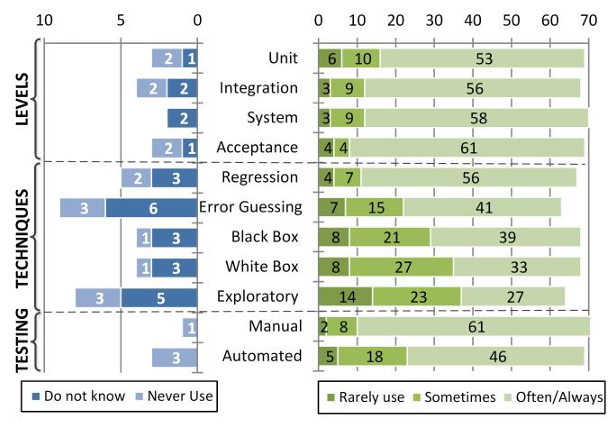
\includegraphics[width=1\linewidth]{figures/tests/frequency_of_use__levels_techniques_and_types_of_testing.png}
    \label{fig:frequency_of_use_levels_techniques_and_types_of_testing}
    \footnotesize Source: \cite{sanchez2020beyond}
\end{figure}

The result shown in the figure \ref{fig:frequency_of_use_levels_techniques_and_types_of_testing}
expresses clearly that integration and unit tests are among the most known and used types of tests. The majority of the interviewed people know about the existence and use of both the black and white box techniques.
And all of them know about automated testing. The result highlighted the importance of the unit and integration tests. As illustrated by the figure \ref{fig:frequency_of_use_levels_techniques_and_types_of_testing},
53\% and 56\% of the developers use unit and integration tests. They, respectively, rank 3rd and 2nd, while acceptance test's rank is 1st.

Another survey conducted by \cite{lee2012survey} revealed that they are among the most used types of automated software tests, as exhibited in the figure \ref{fig:usage_stmt_tests_processes}.

\begin{figure}[H]
    \centering
    \caption{Usage of Software Testing Methods and Tools in Tests Processes}
    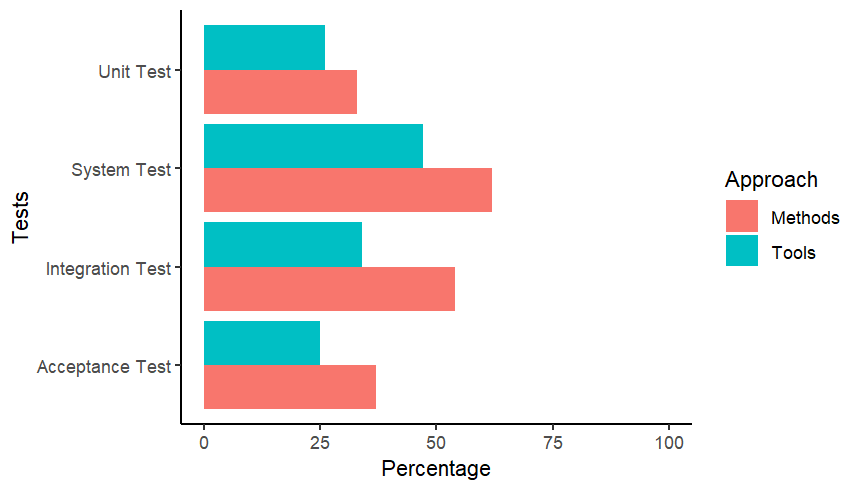
\includegraphics[width=0.8\linewidth]{figures/tests/usage_stmt_tests_processes.png}
    \label{fig:usage_stmt_tests_processes}
    \\ \footnotesize Source: Adapted from \cite{lee2012survey}.
\end{figure}

The result expressed in the figure \ref{fig:usage_stmt_tests_processes}, both unit and integration ranked 4th and 2nd, respectively, while system and acceptance tests ranked 1st and 3rd, respectively. As the last example of a survey, \cite{hynninen2023development} illustrated in the figure \ref{fig:testing_tools_2017_2009} the number of uses of the most used types of tests.

\begin{figure}[H]
    \centering
    \caption{Percentage of the Testing and QA Tools Utilized in the Industry}
    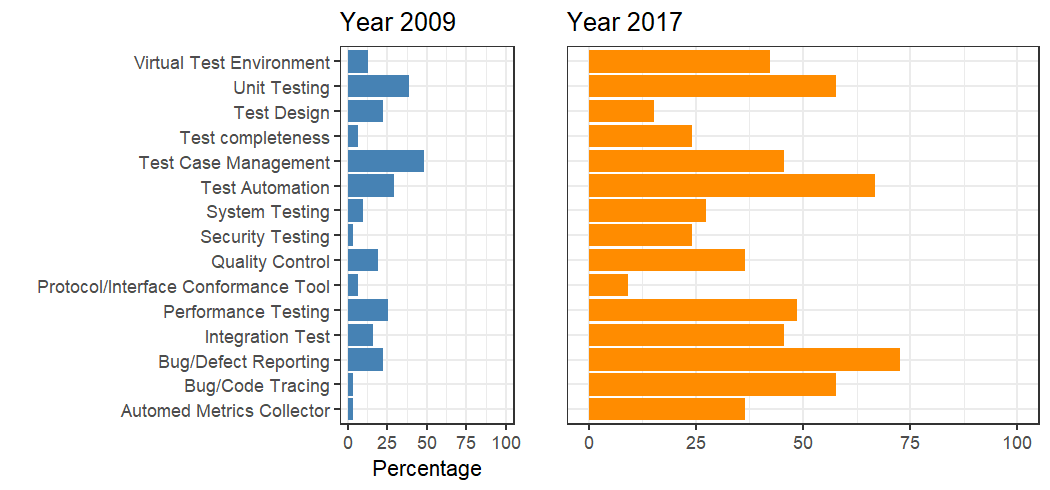
\includegraphics[width=0.8\linewidth]{figures/tests/testing_tools_2017_2009.png}
    \label{fig:testing_tools_2017_2009}
    \\ \footnotesize Source: Adapted from \cite{hynninen2023development, kasurinen2010software}.
\end{figure}

It is notable the dominance of the unit and integration tests in the plot \ref{fig:testing_tools_2017_2009}, ranking 1st and 3rd. Regardless of the ranks of unit and integration tests achieved in the surveys of \cite{hynninen2023development, kasurinen2010software, lee2012survey, sanchez2020beyond}, they are the most used types of automated types of tests. Their importance can be noticed and measured effortlessly via the results of the surveys.

As a consequence, in order to create unit and integration tests executable, test cases are the correct approach. \cite{abo2023role, thant2023impact} define a test case as a collection of input data used to execute the program
under test, whose development is based on the requirements and specifications of the software and designed to cover all possible scenarios and edge cases. 

Consequently, test cases require software testing automation tools to execute the planned tests. \cite{umar2019study} defines the categories of software testing automation tools as follows: unit testing tools, functional testing tools, code coverage tools, test management tools, and performance testing tools.

Specially, the goal of functional testing of a software system is to find discrepancies between the actual behavior of the implemented system’s functions and the desired behavior as described in the system’s functional specification \cite{ostrand_balcer_1988}.

Considering all the paragraphs's information in this subsection, the unit and integration tests were the types of tests selected to be used in this work.

A unit test scrutinizes the behavior of an individual, self-contained unit of work. In Java applications, this \textit{distinct unit of work} frequently, though not exclusively, corresponds to a single method. In contrast, integration and acceptance tests evaluate the interactions between different components. A unit of work is defined as a task that can be executed independently of other tasks. Consequently, unit tests often concentrate on verifying if a method adheres to the specifications outlined in its API contract \cite{massol2004junit}.

For unit tests, among the types of automation tools cited by  \cite{umar2019study}, \hyperref[appendix:glossary]{JUnit} was the chosen framework. The figure \ref{tab:junit_comparison_advantages_disadvantages} displays the comparison between the advantages and disadvantages of \hyperref[appendix:glossary]{JUnit}.

\begin{table}[h]
    \centering
    \caption{Comparison of Advantages and Disadvantages of JUnit}
    \label{tab:junit_comparison_advantages_disadvantages}
    \begin{tabular}{p{0.45\textwidth} p{0.45\textwidth}}
        \hline
        \textbf{Advantages} & \textbf{Disadvantages} \\
        \hline
        Facilitates changes and simplifies integration & Requires programming skills and consumes time to write and check. \\
        \hline
        Bugs can be found and resolved early without affecting other pieces of the code. & It can only run tests on one JVM, as such developers are unable to test applications that require multiple JVMs. \\
        \hline
    \end{tabular}
    \footnotesize Source: Adapted from \cite{umar2019study}.
\end{table}

It is notable how the advantages overcome the disadvantages. In addition, for integration tests, \textit{MockMvc} shall be the chosen framework. 
Complementing the paragraphs above, all integration tests shall use the following annotations present in the table \ref{table:integration_tests_annotations}.

\begin{table}[H]
\centering
\caption{Spring Boot Testing Annotations and Components}
\label{table:integration_tests_annotations}
\begin{tabular}{p{0.25\textwidth}p{0.7\textwidth}}
\toprule
\textbf{Name} & \textbf{Description} \\
\midrule
@SpringBootTest & Specifies that a test class runs Spring Boot based tests. \\ \hline
@TestMethodOrderer & A type-level annotation used to configure a MethodOrderer for the test methods of the annotated test class or test interface. \\ \hline
@MethodOrderer & Defines the API for ordering the test methods in a given test class. \\ \hline
@Test & Used to signal that the annotated method is a test method. \\ \hline
@Order & An annotation used to configure the order in which the annotated element should be evaluated or executed relative to other elements of the same category. \\
\bottomrule
\end{tabular}
\footnotesize Source: Adapted from \cite{junit5_methodorderer_api, junit5_order_api, junit5_test_api, junit5testmethodorder_api, springboottest_api}.
\end{table}

They are examples of methods of integration tests that use the annotations present in the table \ref{table:integration_tests_annotations} the figures \ref{fig:medical_slot_successful_registration_example},
\ref{fig:medical_slot_unsuccessful_registration_duplicated_datetime},
and \ref{fig:medical_slot_unsuccessful_registration_not_found_doctor}. The first figure illustrates an example of a success-oriented testing method that registers a medical slot.

\begin{figure}[H]
    \centering
    \caption{Example of a Customer Successful Registration Testing Method}
    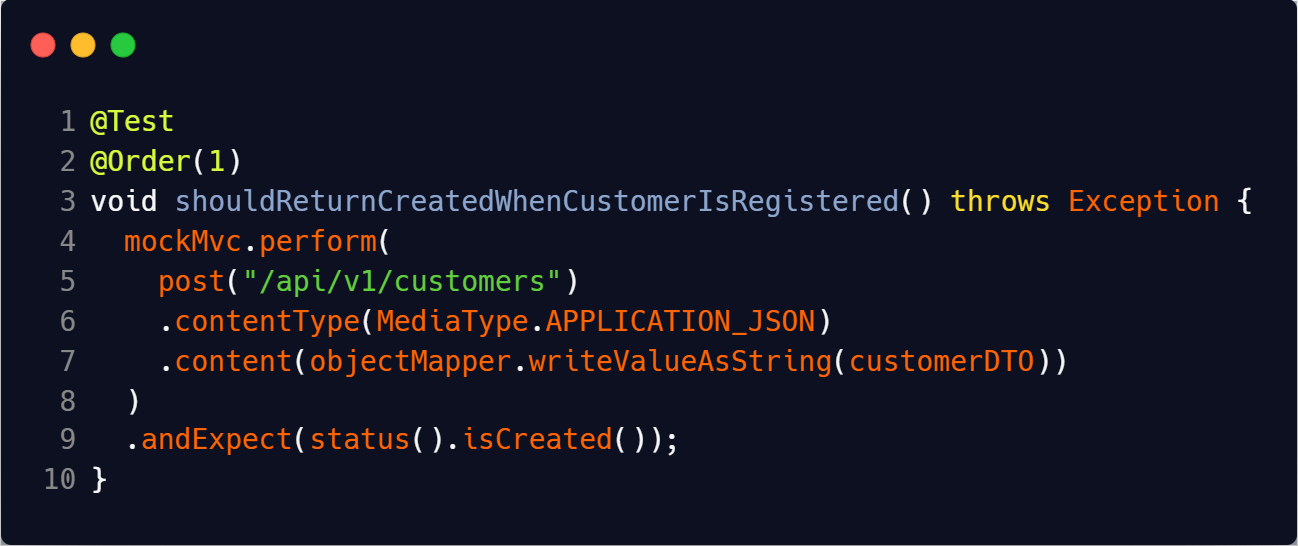
\includegraphics[width=1\linewidth]{figures/tests/customer_successful_registration_example.png}
    \footnotesize Source: Author's creation.
    \label{fig:customer_successful_registration_example}
\end{figure}

The method of the figure \ref{fig:customer_successful_registration_example} returns the \hyperref[tab:summary_http_status_codes]{status code 201}. In contrast with this method, there is the figure \ref{fig:customer_unsuccessful_registration_duplicated_sin}.

\begin{figure}[H]
    \centering
    \caption{Example of Customer Unsuccessful Registration Testing Method - Duplicated SIN}
    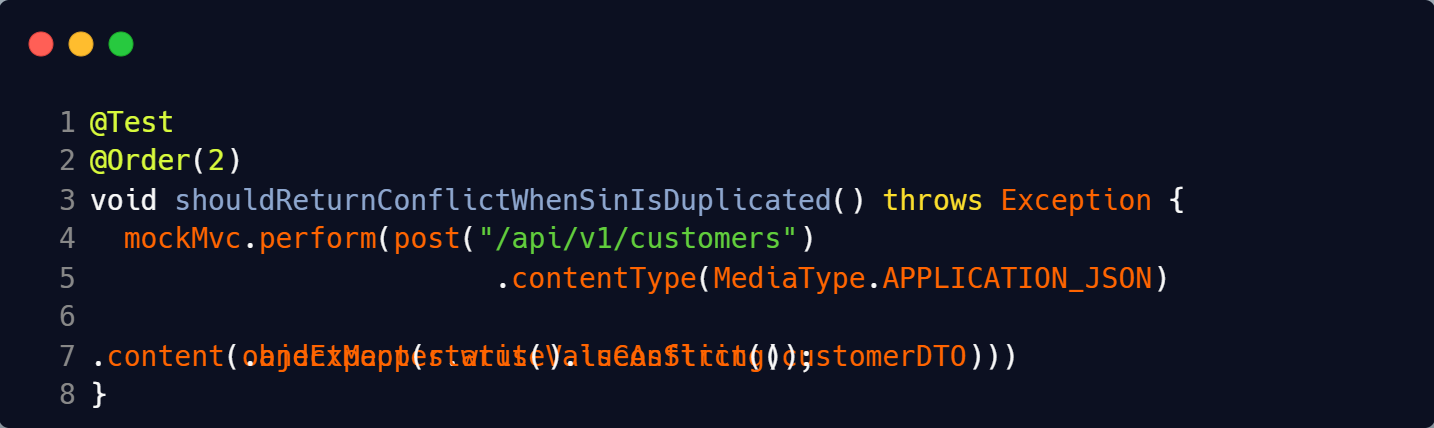
\includegraphics[width=1\linewidth]{figures/tests/customer_unsuccessful_registration_duplicated_sin.PNG}
    \footnotesize Source: Author's creation.
    \label{fig:customer_unsuccessful_registration_duplicated_sin}
\end{figure}

The figure \ref{fig:medical_slot_unsuccessful_registration_duplicated_datetime} illustrates an unsuccessful-oriented testing method that blocks a medical slot due to a booking date and time that is in use in an active medical slot. The method of the figure \ref{fig:medical_slot_unsuccessful_registration_duplicated_datetime} returns the \hyperref[tab:summary_http_status_codes]{status code 409}.


Considering all the figures \ref{fig:medical_slot_successful_registration_example}, \ref{fig:medical_slot_unsuccessful_registration_duplicated_datetime}, the methods illustrated inside them all have in common the annotations \textit{@Order} and \textit{@Test} and an instance of the framework \textit{WebTestClient}. They are all using the annotations mentioned in the table \ref{table:integration_tests_annotations}. 

Finally, the use of the mentioned annotations created the perfect and functional environment for integration tests. As an example, the annotation \textit{@SpringBootTest} can select a random port to avoid the use of the standard port (e.g., \textit{8080:8080}). This prevents the API from having unexpected behaviors that interrupt the application ungracefully. Similar to the previous explanation, the annotation \textit{@Order} derives from the annotation \textit{@TestMethodOrder} that enables its ordering ability of setting the execution order of the test methods. One benefit of setting the execution order is barring occurrences when the successful-oriented method is executed after one of the unsuccessful-oriented ones, which blurs the test's result, if the tester is not aware of such an error.
